RTMが出力した連続値の犯罪発生リスクを,
平均未満,平均以上1標準偏差未満,1標準偏差以上2標準偏差未満,2標準偏差以上の4カテゴリーに分割した.
4カテゴリーの混同行列作成し,各グリッドセルの犯罪発生リスクをリスクマップとして地図上にを図示した.

また,RTMが出力した高リスクと低リスクの2カテゴリーから混同行列を作成し,
False Positive(FP)・False Negative(FN)のグリッドセルを地図上に図示する.

2011年〜2013年でモデルを学習し,2014年で評価した結果を示す.
2014年に実際に起った強盗犯罪の発生地点とそれに基づいた実際のリスクマップを
図\ref{fig:non-crime-no-timeseries-actual-risk}に示す.
DFによるリスクマップを図\ref{fig:non-crime-no-timeseries-df-risk}に,
CFによるリスクマップを図\ref{fig:non-crime-no-timeseries-cf-risk}に,
NEによるリスクマップを図\ref{fig:non-crime-no-timeseries-ne-risk}に,
LDによるリスクマップを図\ref{fig:non-crime-no-timeseries-ld-risk}に,
GFによるリスクマップを図\ref{fig:non-crime-no-timeseries-gf-risk}に,
TGによるリスクマップを図\ref{fig:non-crime-no-timeseries-tg-risk}に,
GF+TGによるリスクマップを図\ref{fig:non-crime-no-timeseries-gf-tg-risk}に
示す.
実際のリスクマップと比べて,DFによるリスクマップでは高い空間相関を持つが,
CF,NE,LD,GFによるリスクマップは空間相関が削減された.
また,TGでは若干の空間相関を持つがGF+TGでは空間相関が削減された.


また,
4カテゴリーの混同行列を図\ref{fig:non-crime-no-timeseries-4cm}に,
2カテゴリーの混同行列を図\ref{fig:non-crime-no-timeseries-2cm}に,
各モデルによるFP・FNのグリッドセルを
図\ref{fig:non-crime-no-timeseries-df-fnp}から
図\ref{fig:non-crime-no-timeseries-gf-tg-fnp}に示した.

%------------------------------------------
% risk map
%------------------------------------------
\begin{figure}
  \centering % 図を中央寄せにする
  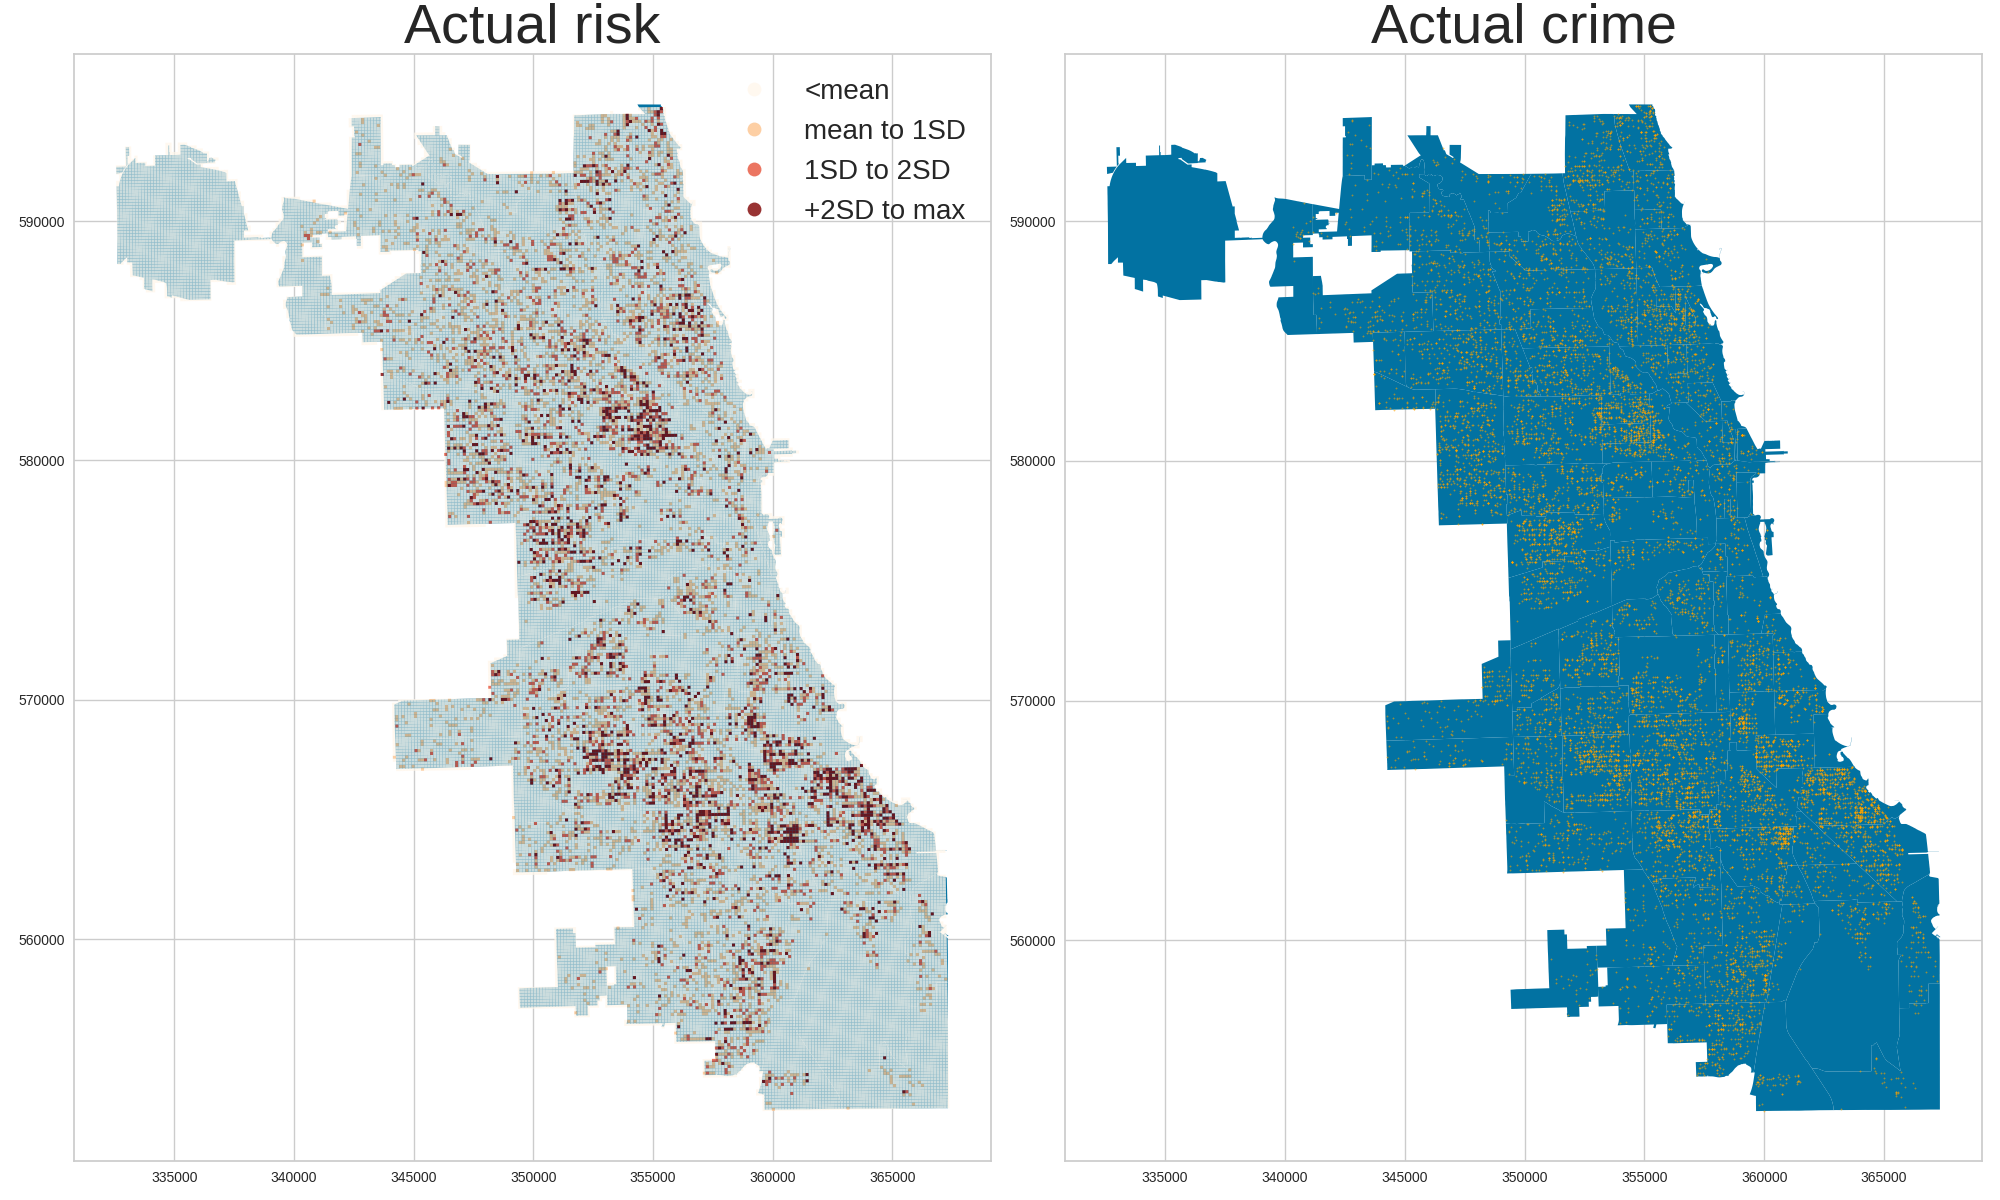
\includegraphics[scale=0.25]{./non-crime-no-timeseries-fig/actual_risk_point_map.png}
  \caption{左:実際のリスクマップ 右:実際の強盗犯罪発生地点}
  \label{fig:non-crime-no-timeseries-actual-risk}
\end{figure}

\begin{figure}
  \centering % 図を中央寄せにする
  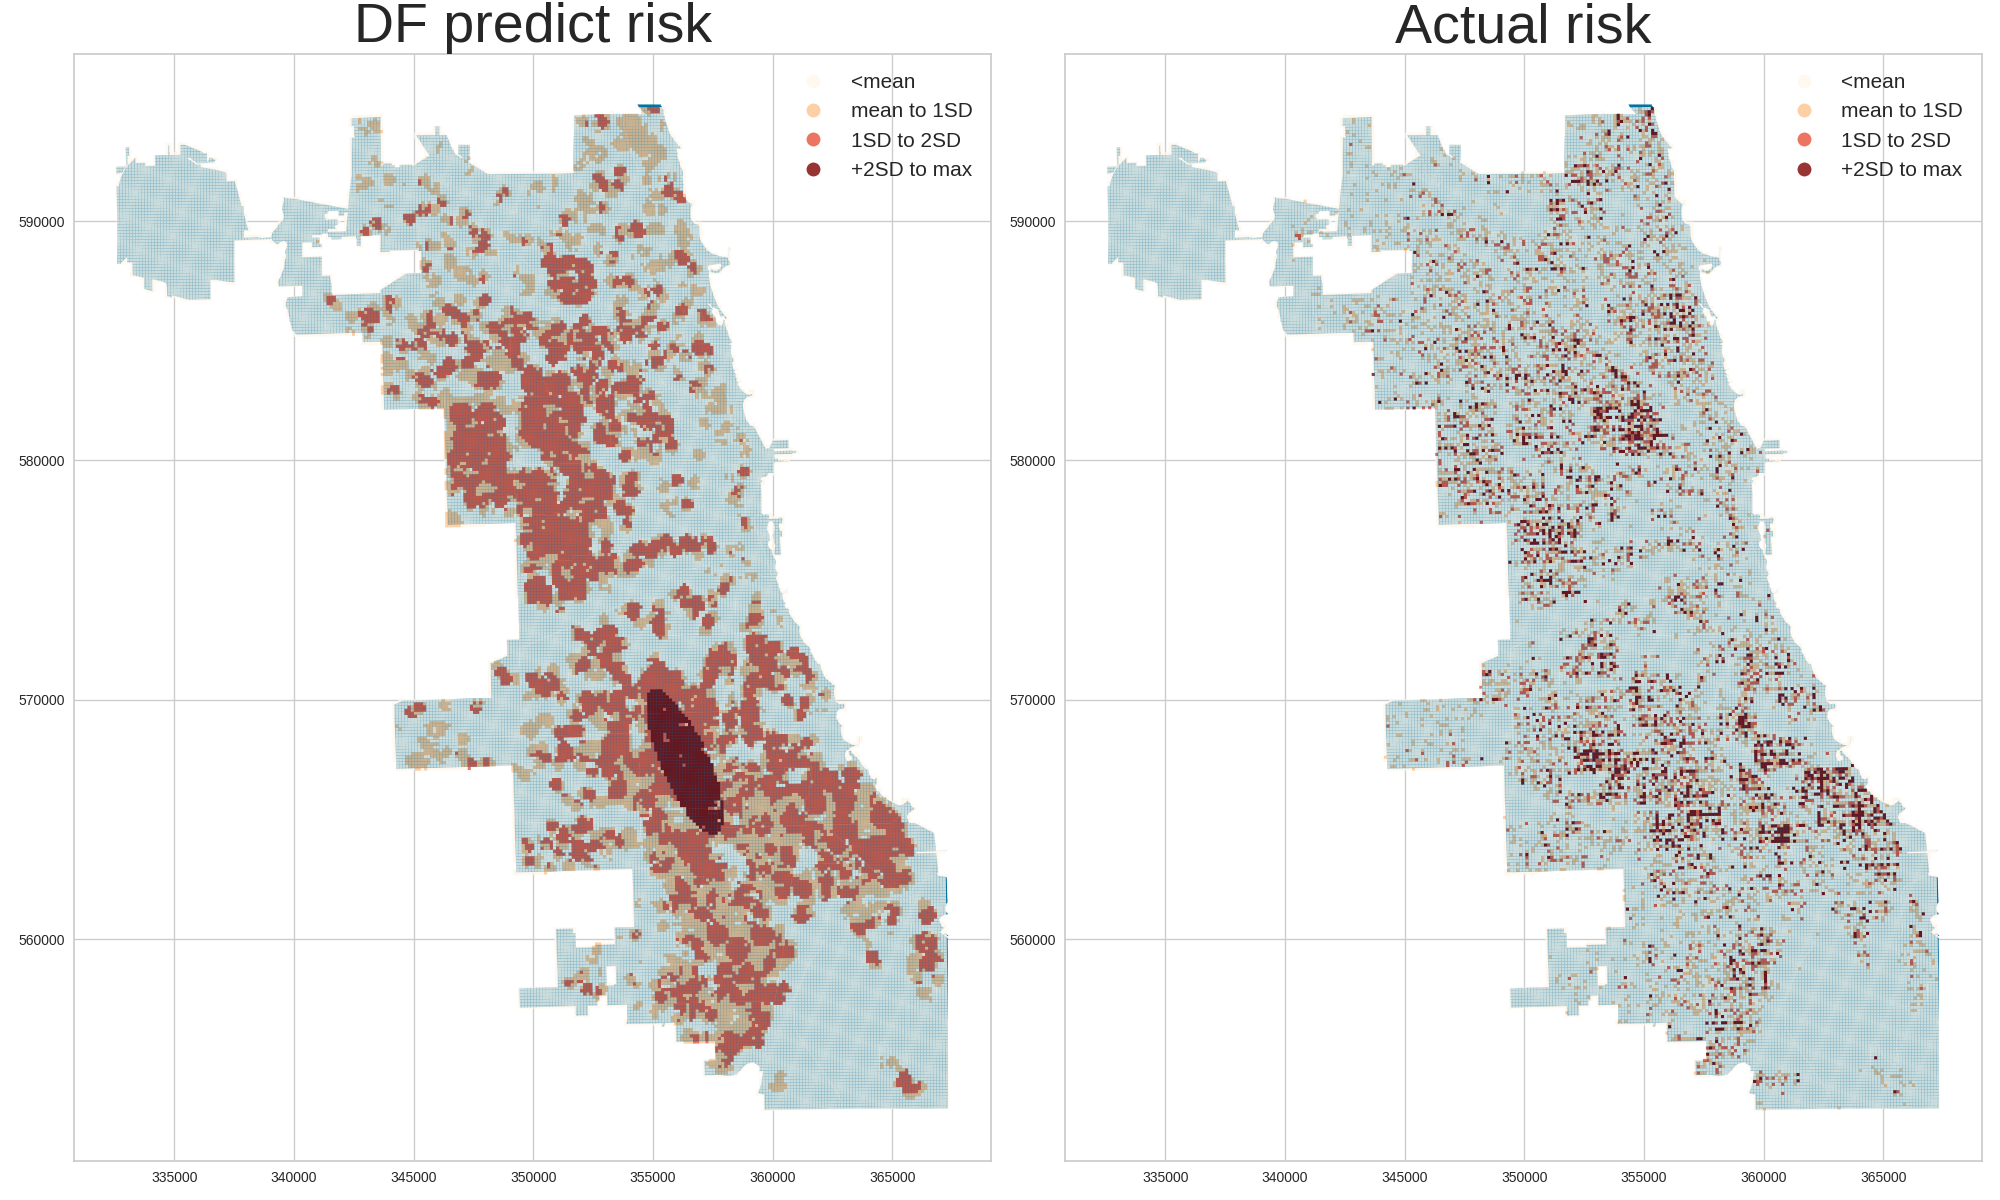
\includegraphics[scale=0.25]{./non-crime-no-timeseries-fig/DF_riskmap.png}
  \caption{左:DFによるリスクマップ 右:実際のリスクマップ}
  \label{fig:non-crime-no-timeseries-df-risk}
\end{figure}

\begin{figure}
  \centering % 図を中央寄せにする
  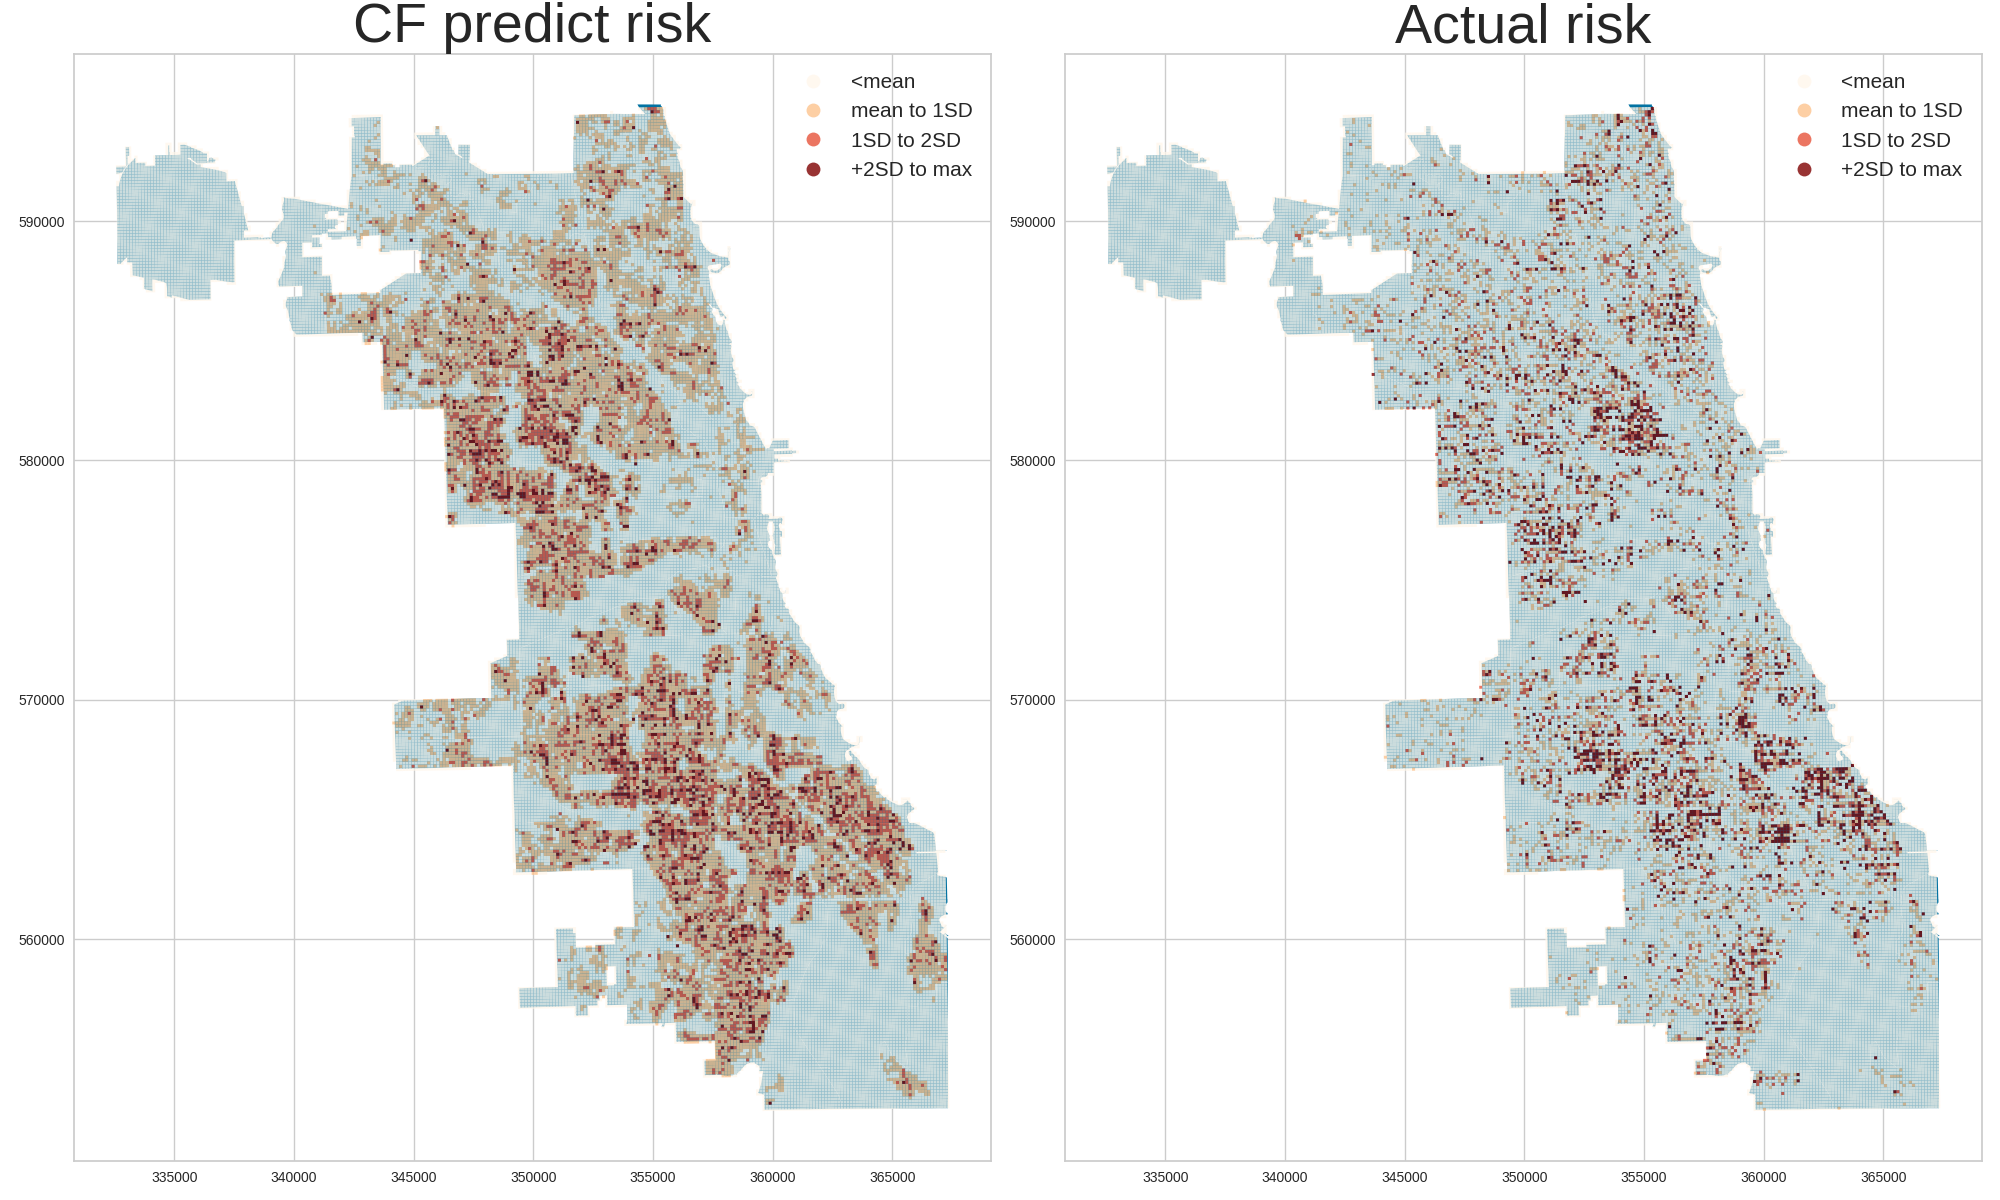
\includegraphics[scale=0.25]{./non-crime-no-timeseries-fig/CF_riskmap.png}
  \caption{左:CFによるリスクマップ 右:実際のリスクマップ}
  \label{fig:non-crime-no-timeseries-cf-risk}
\end{figure}

\begin{figure}
  \centering % 図を中央寄せにする
  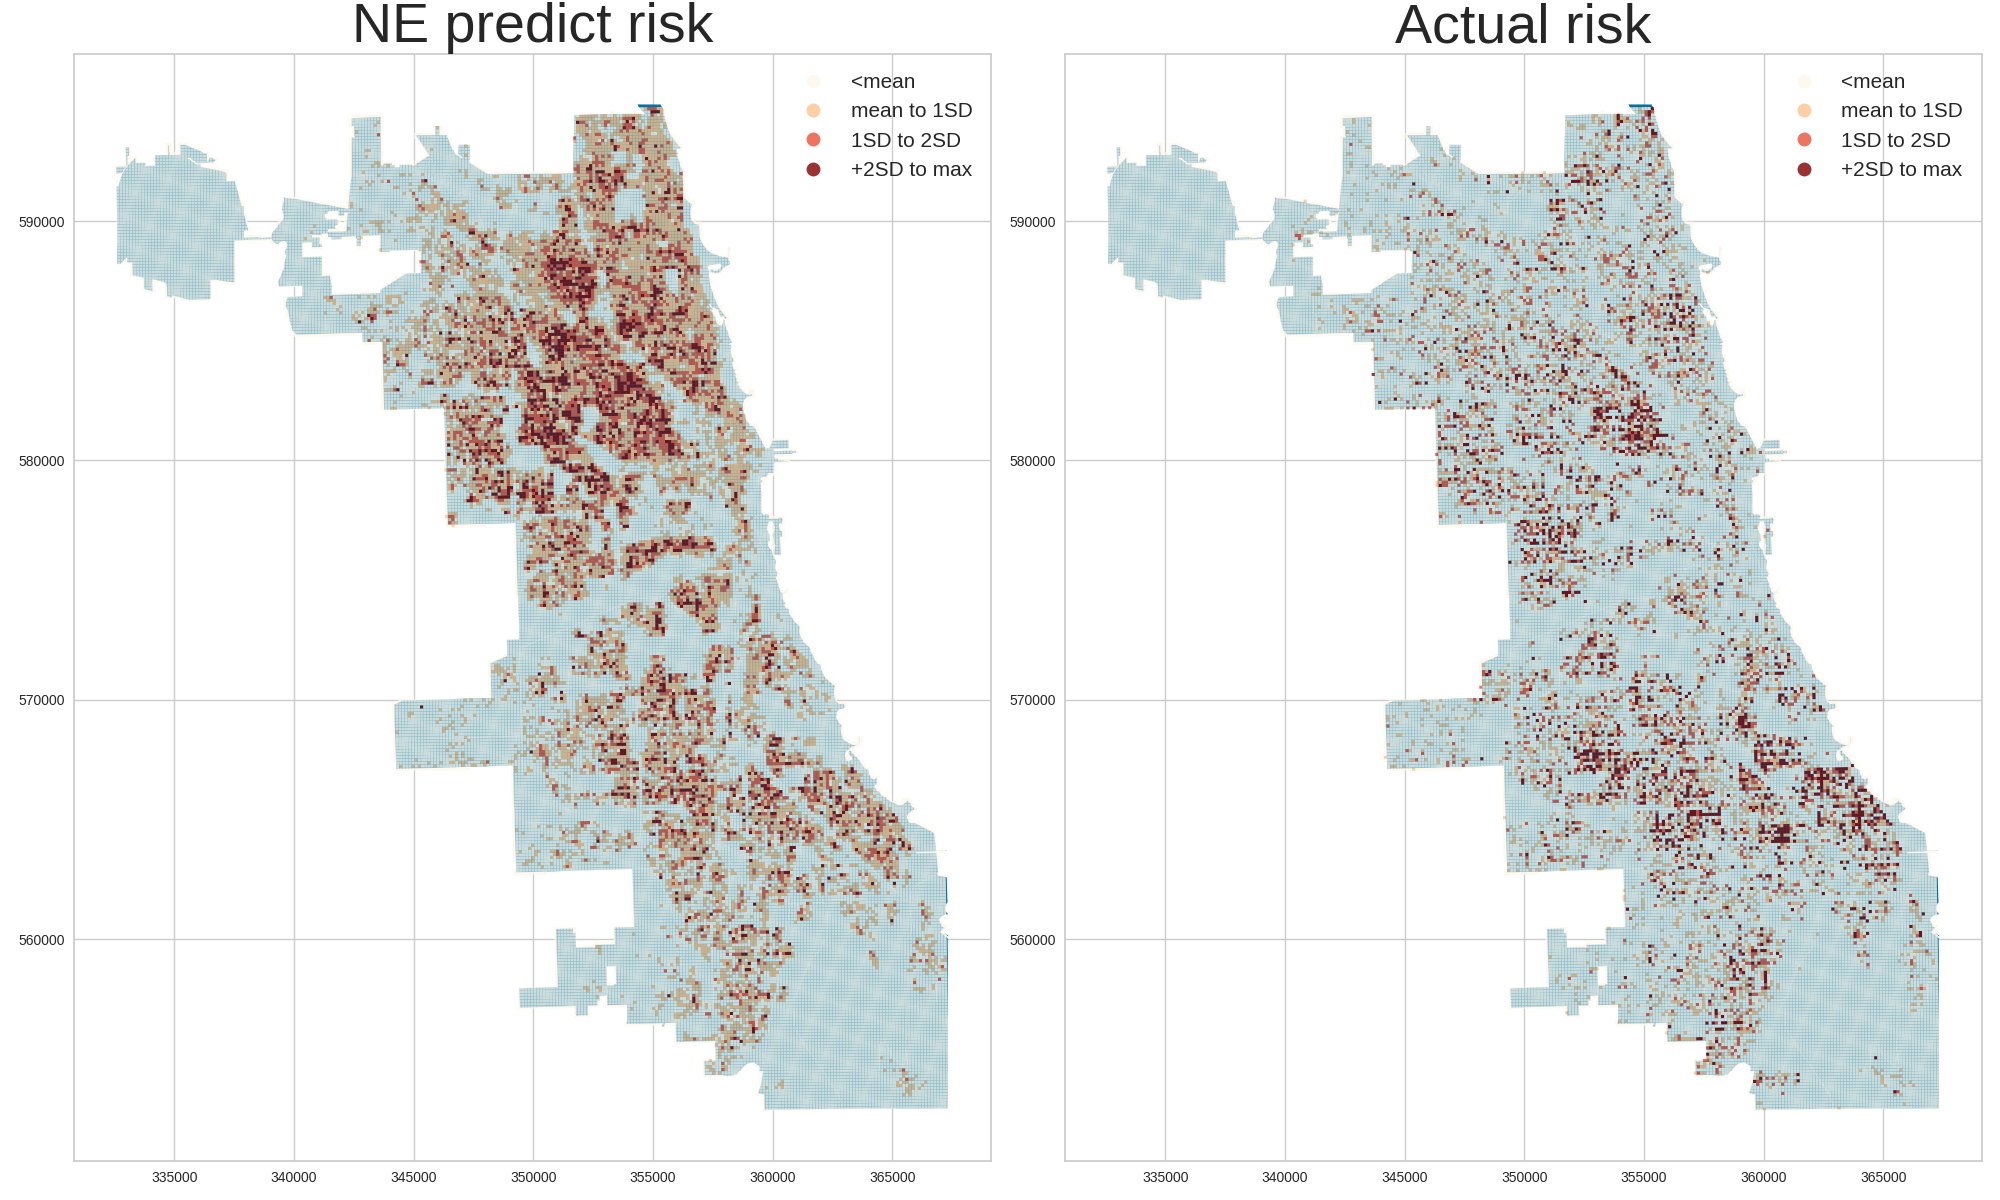
\includegraphics[scale=0.25]{./non-crime-no-timeseries-fig/NE_riskmap.png}
  \caption{左:NEによるリスクマップ 右:実際のリスクマップ}
  \label{fig:non-crime-no-timeseries-ne-risk}
\end{figure}

\begin{figure}
  \centering % 図を中央寄せにする
  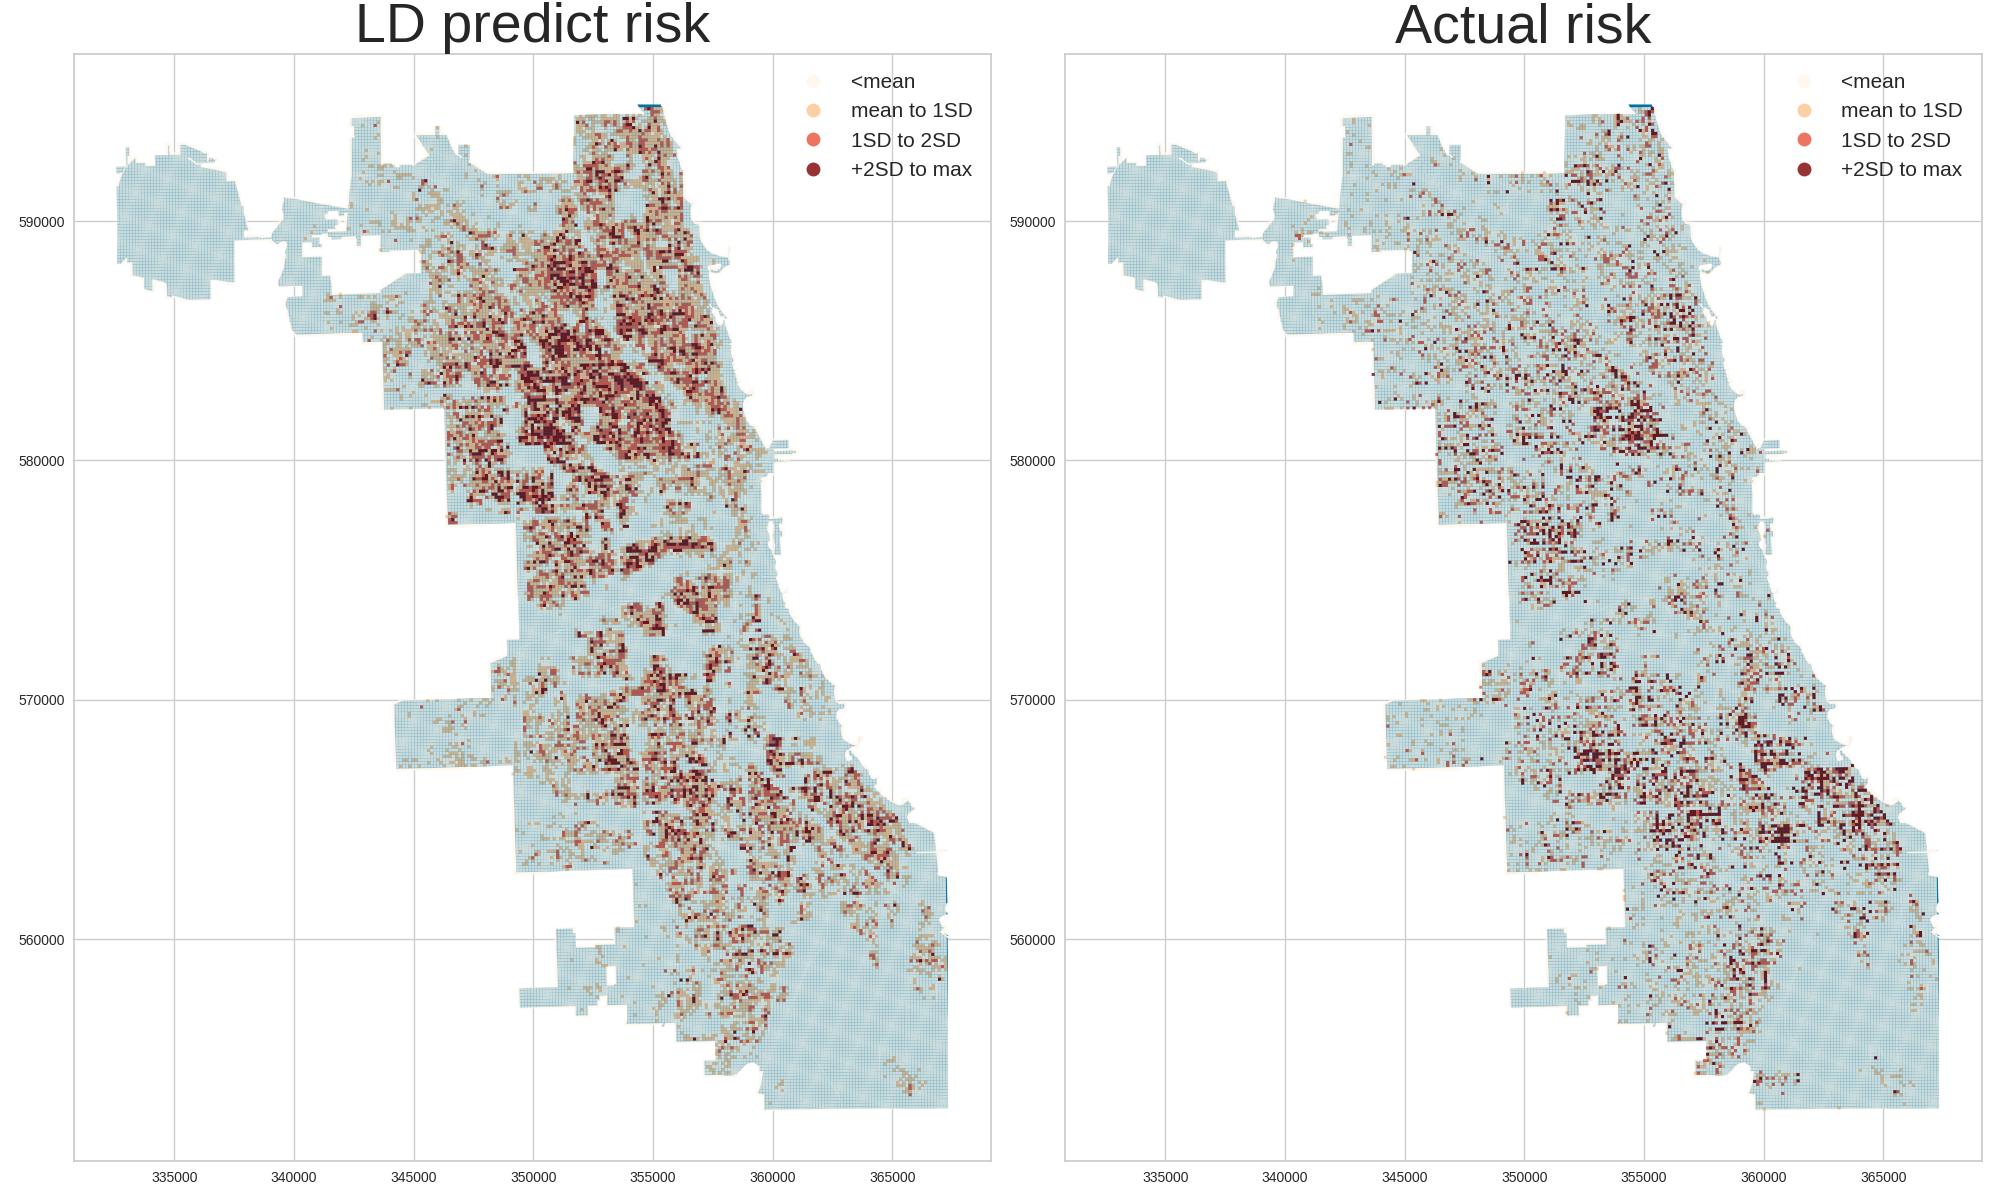
\includegraphics[scale=0.25]{./non-crime-no-timeseries-fig/LD_riskmap.png}
  \caption{左:LDによるリスクマップ 右:実際のリスクマップ}
  \label{fig:non-crime-no-timeseries-ld-risk}
\end{figure}

\begin{figure}
  \centering % 図を中央寄せにする
  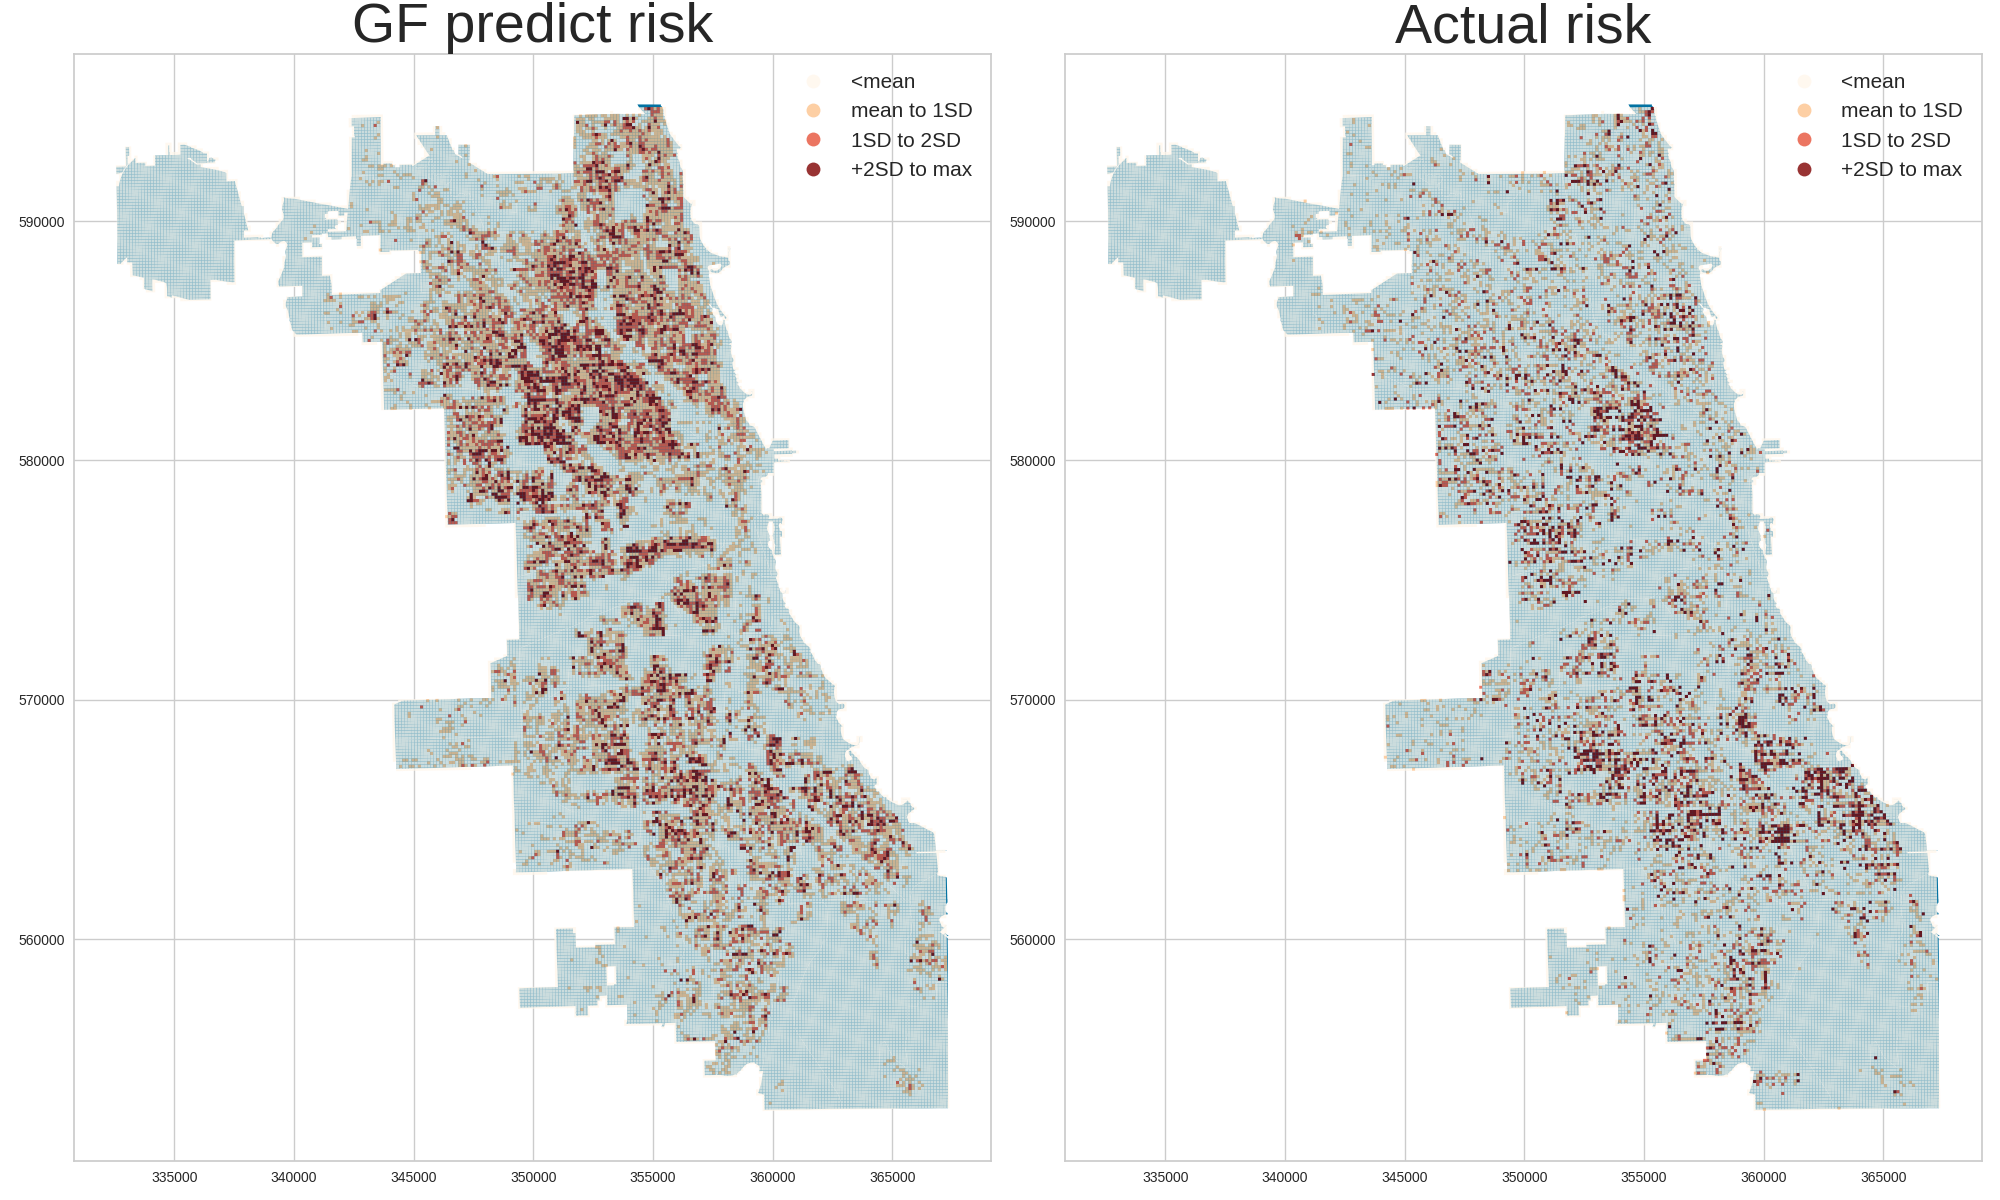
\includegraphics[scale=0.25]{./non-crime-no-timeseries-fig/GF_riskmap.png}
  \caption{左:GFによるリスクマップ 右:実際のリスクマップ}
  \label{fig:non-crime-no-timeseries-gf-risk}
\end{figure}

\begin{figure}
  \centering % 図を中央寄せにする
  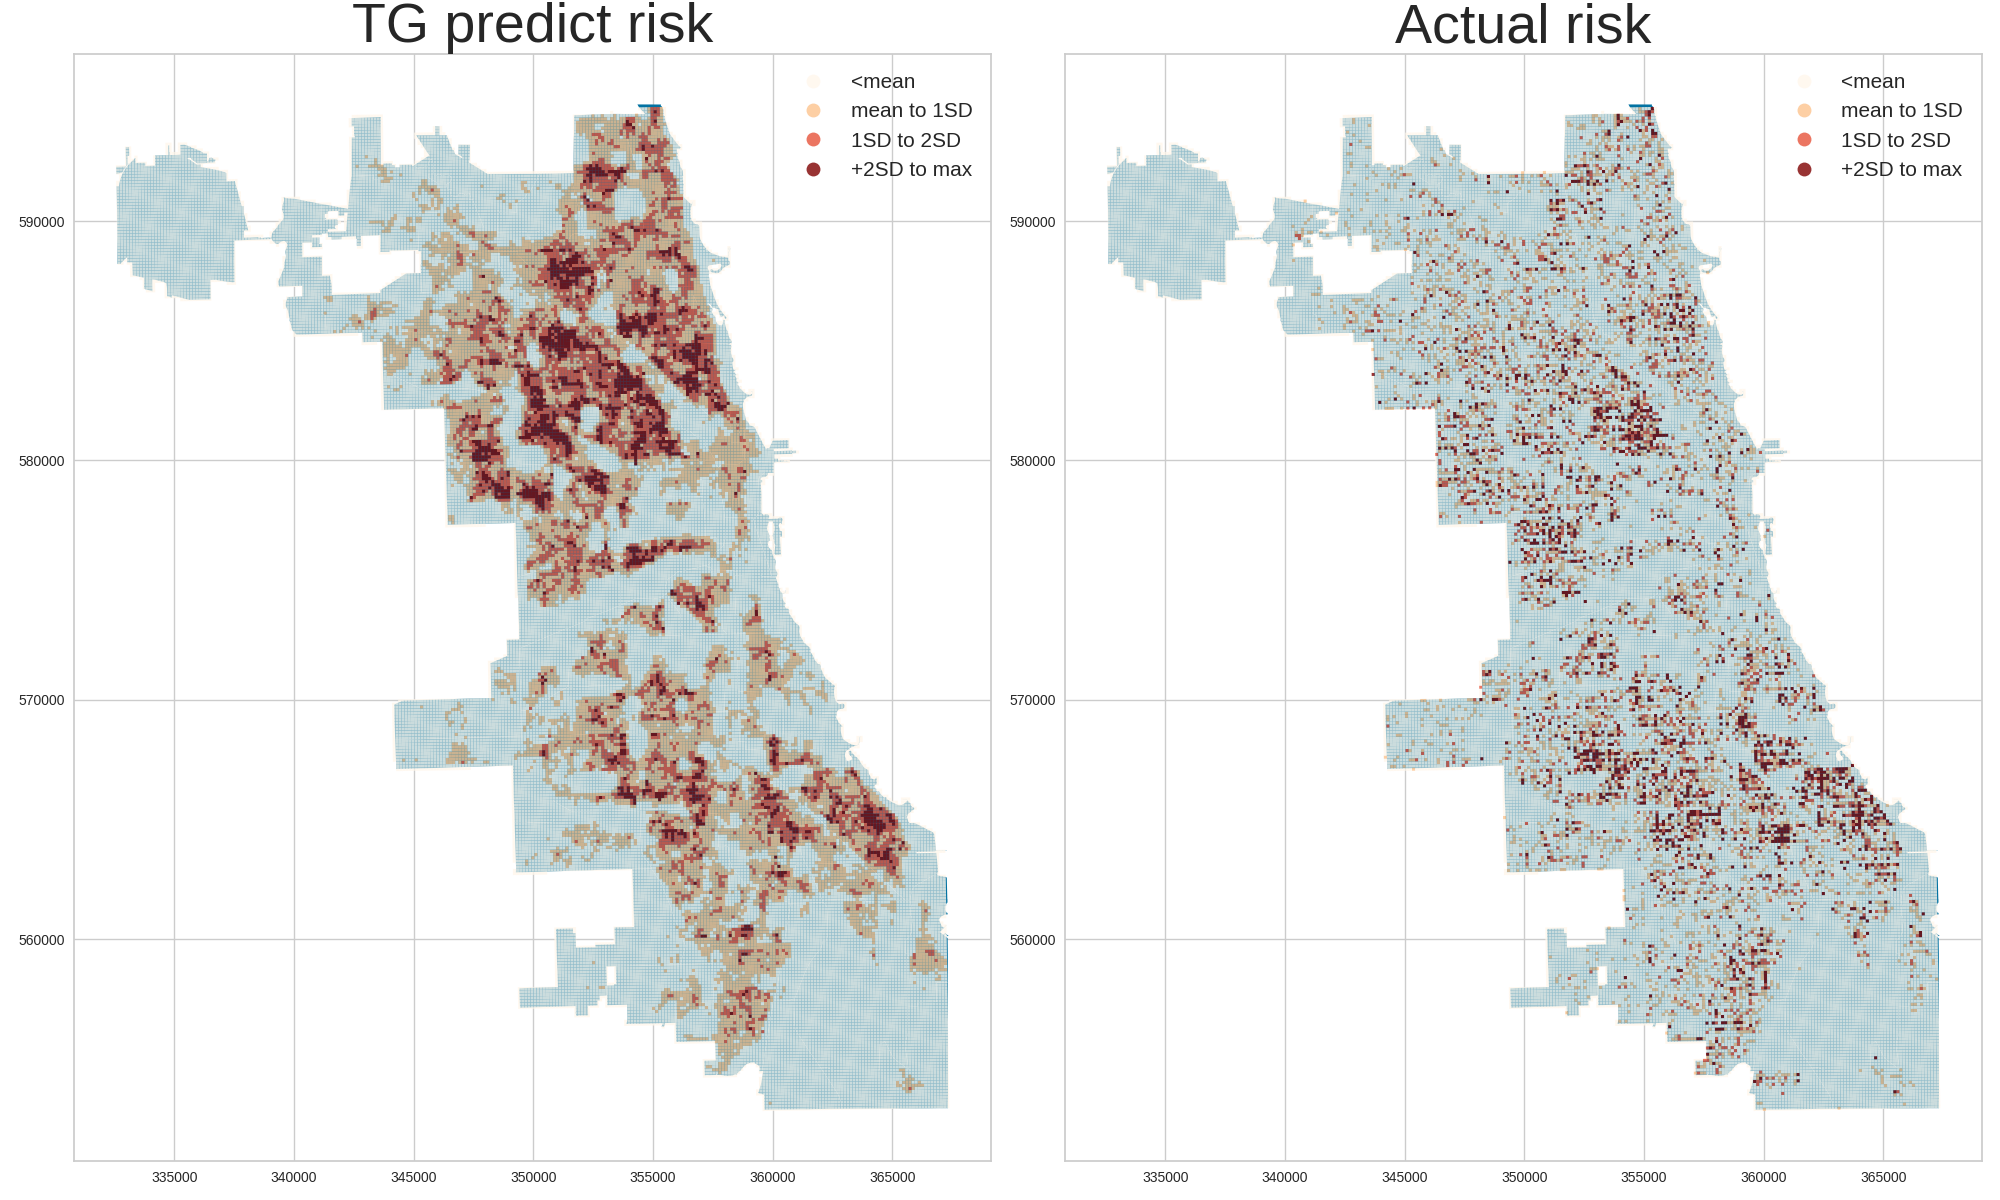
\includegraphics[scale=0.25]{./non-crime-no-timeseries-fig/TG_riskmap.png}
  \caption{左:TGによるリスクマップ 右:実際のリスクマップ}
  \label{fig:non-crime-no-timeseries-tg-risk}
\end{figure}

\begin{figure}
  \centering % 図を中央寄せにする
  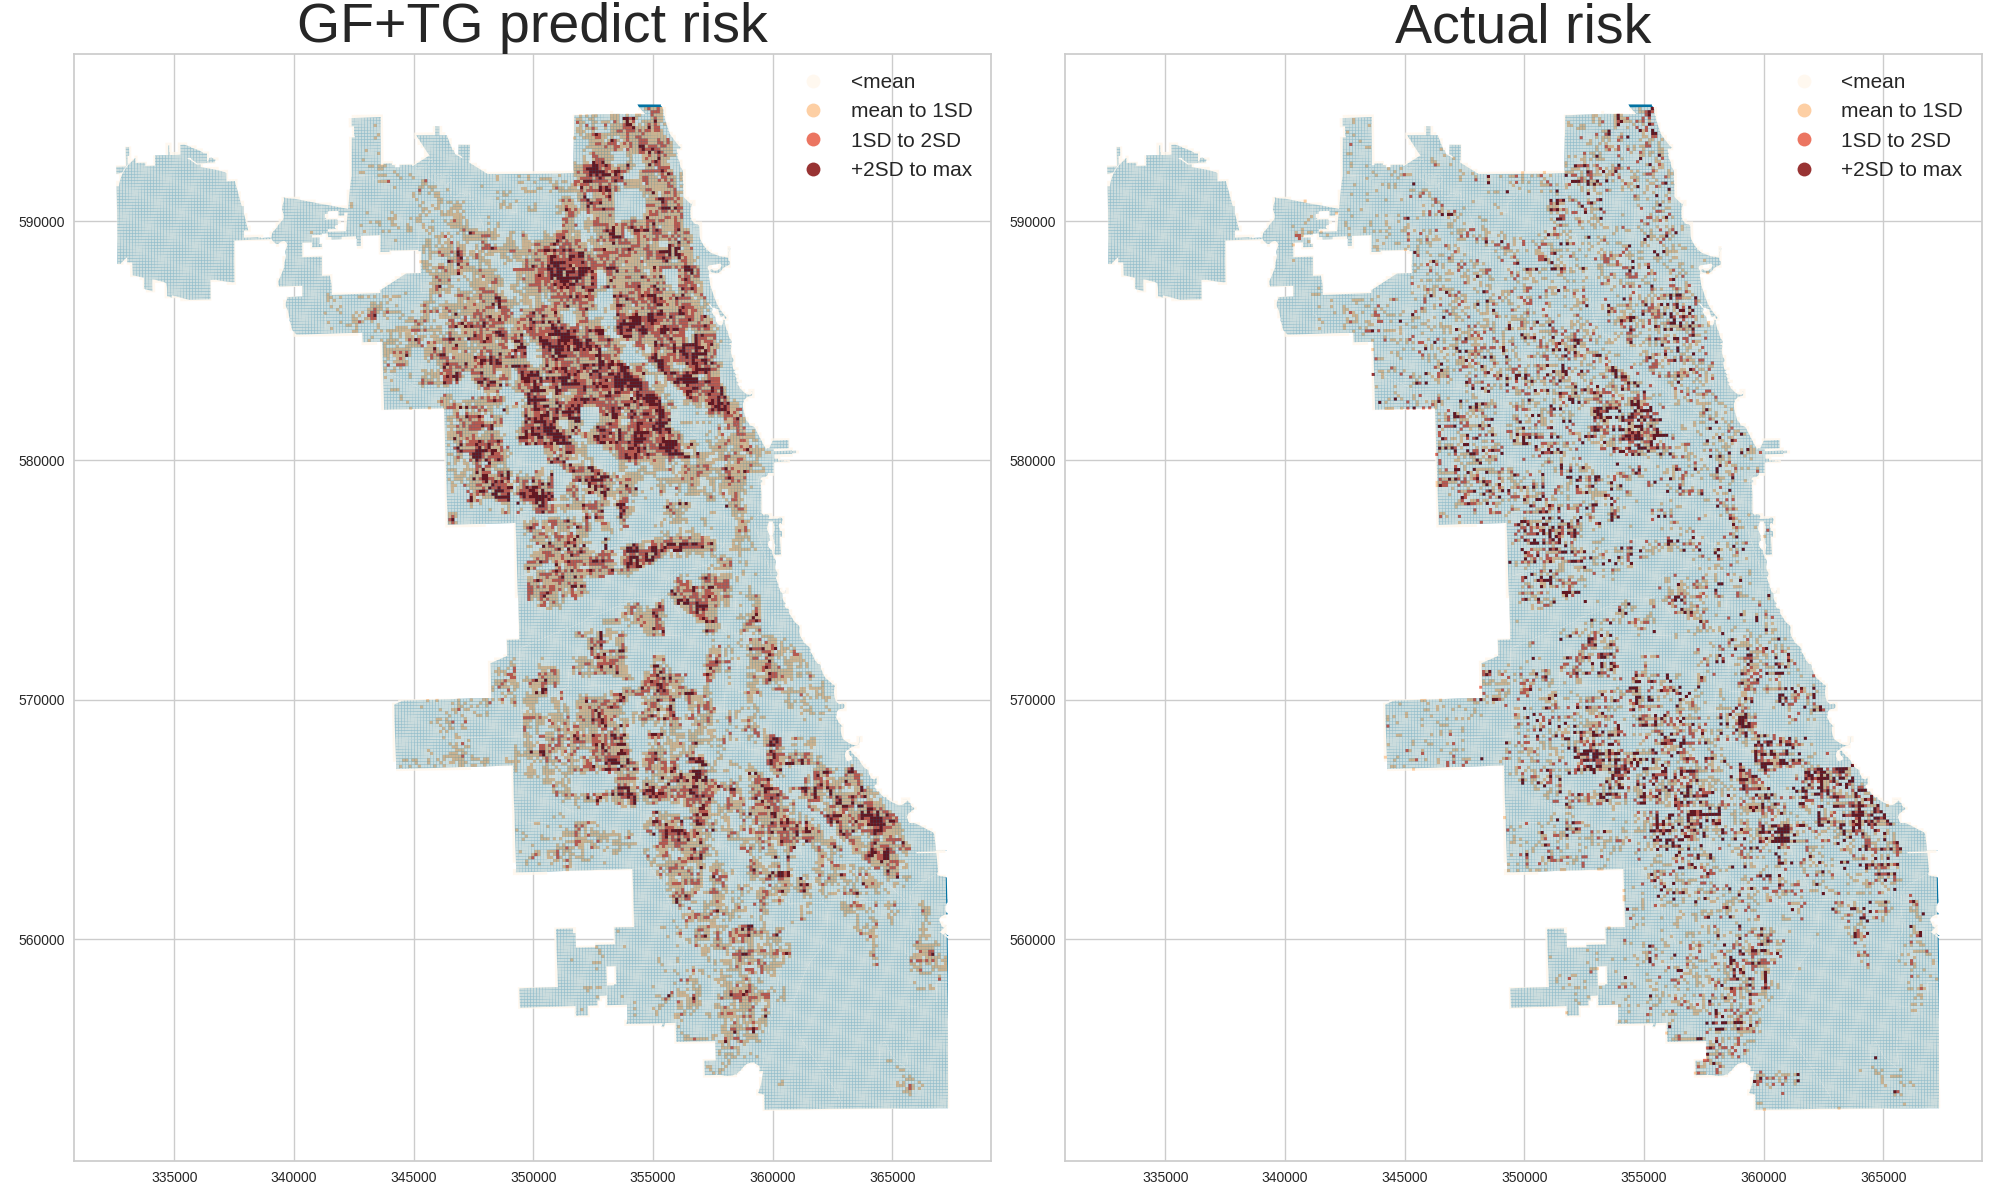
\includegraphics[scale=0.25]{./non-crime-no-timeseries-fig/GF+TG_riskmap.png}
  \caption{左:FG+TGによるリスクマップ 右:実際のリスクマップ}
  \label{fig:non-crime-no-timeseries-gf-tg-risk}
\end{figure}
%------------------------------------------
% confusion matrix
%------------------------------------------
\begin{figure}
  \centering % 図を中央寄せにする
  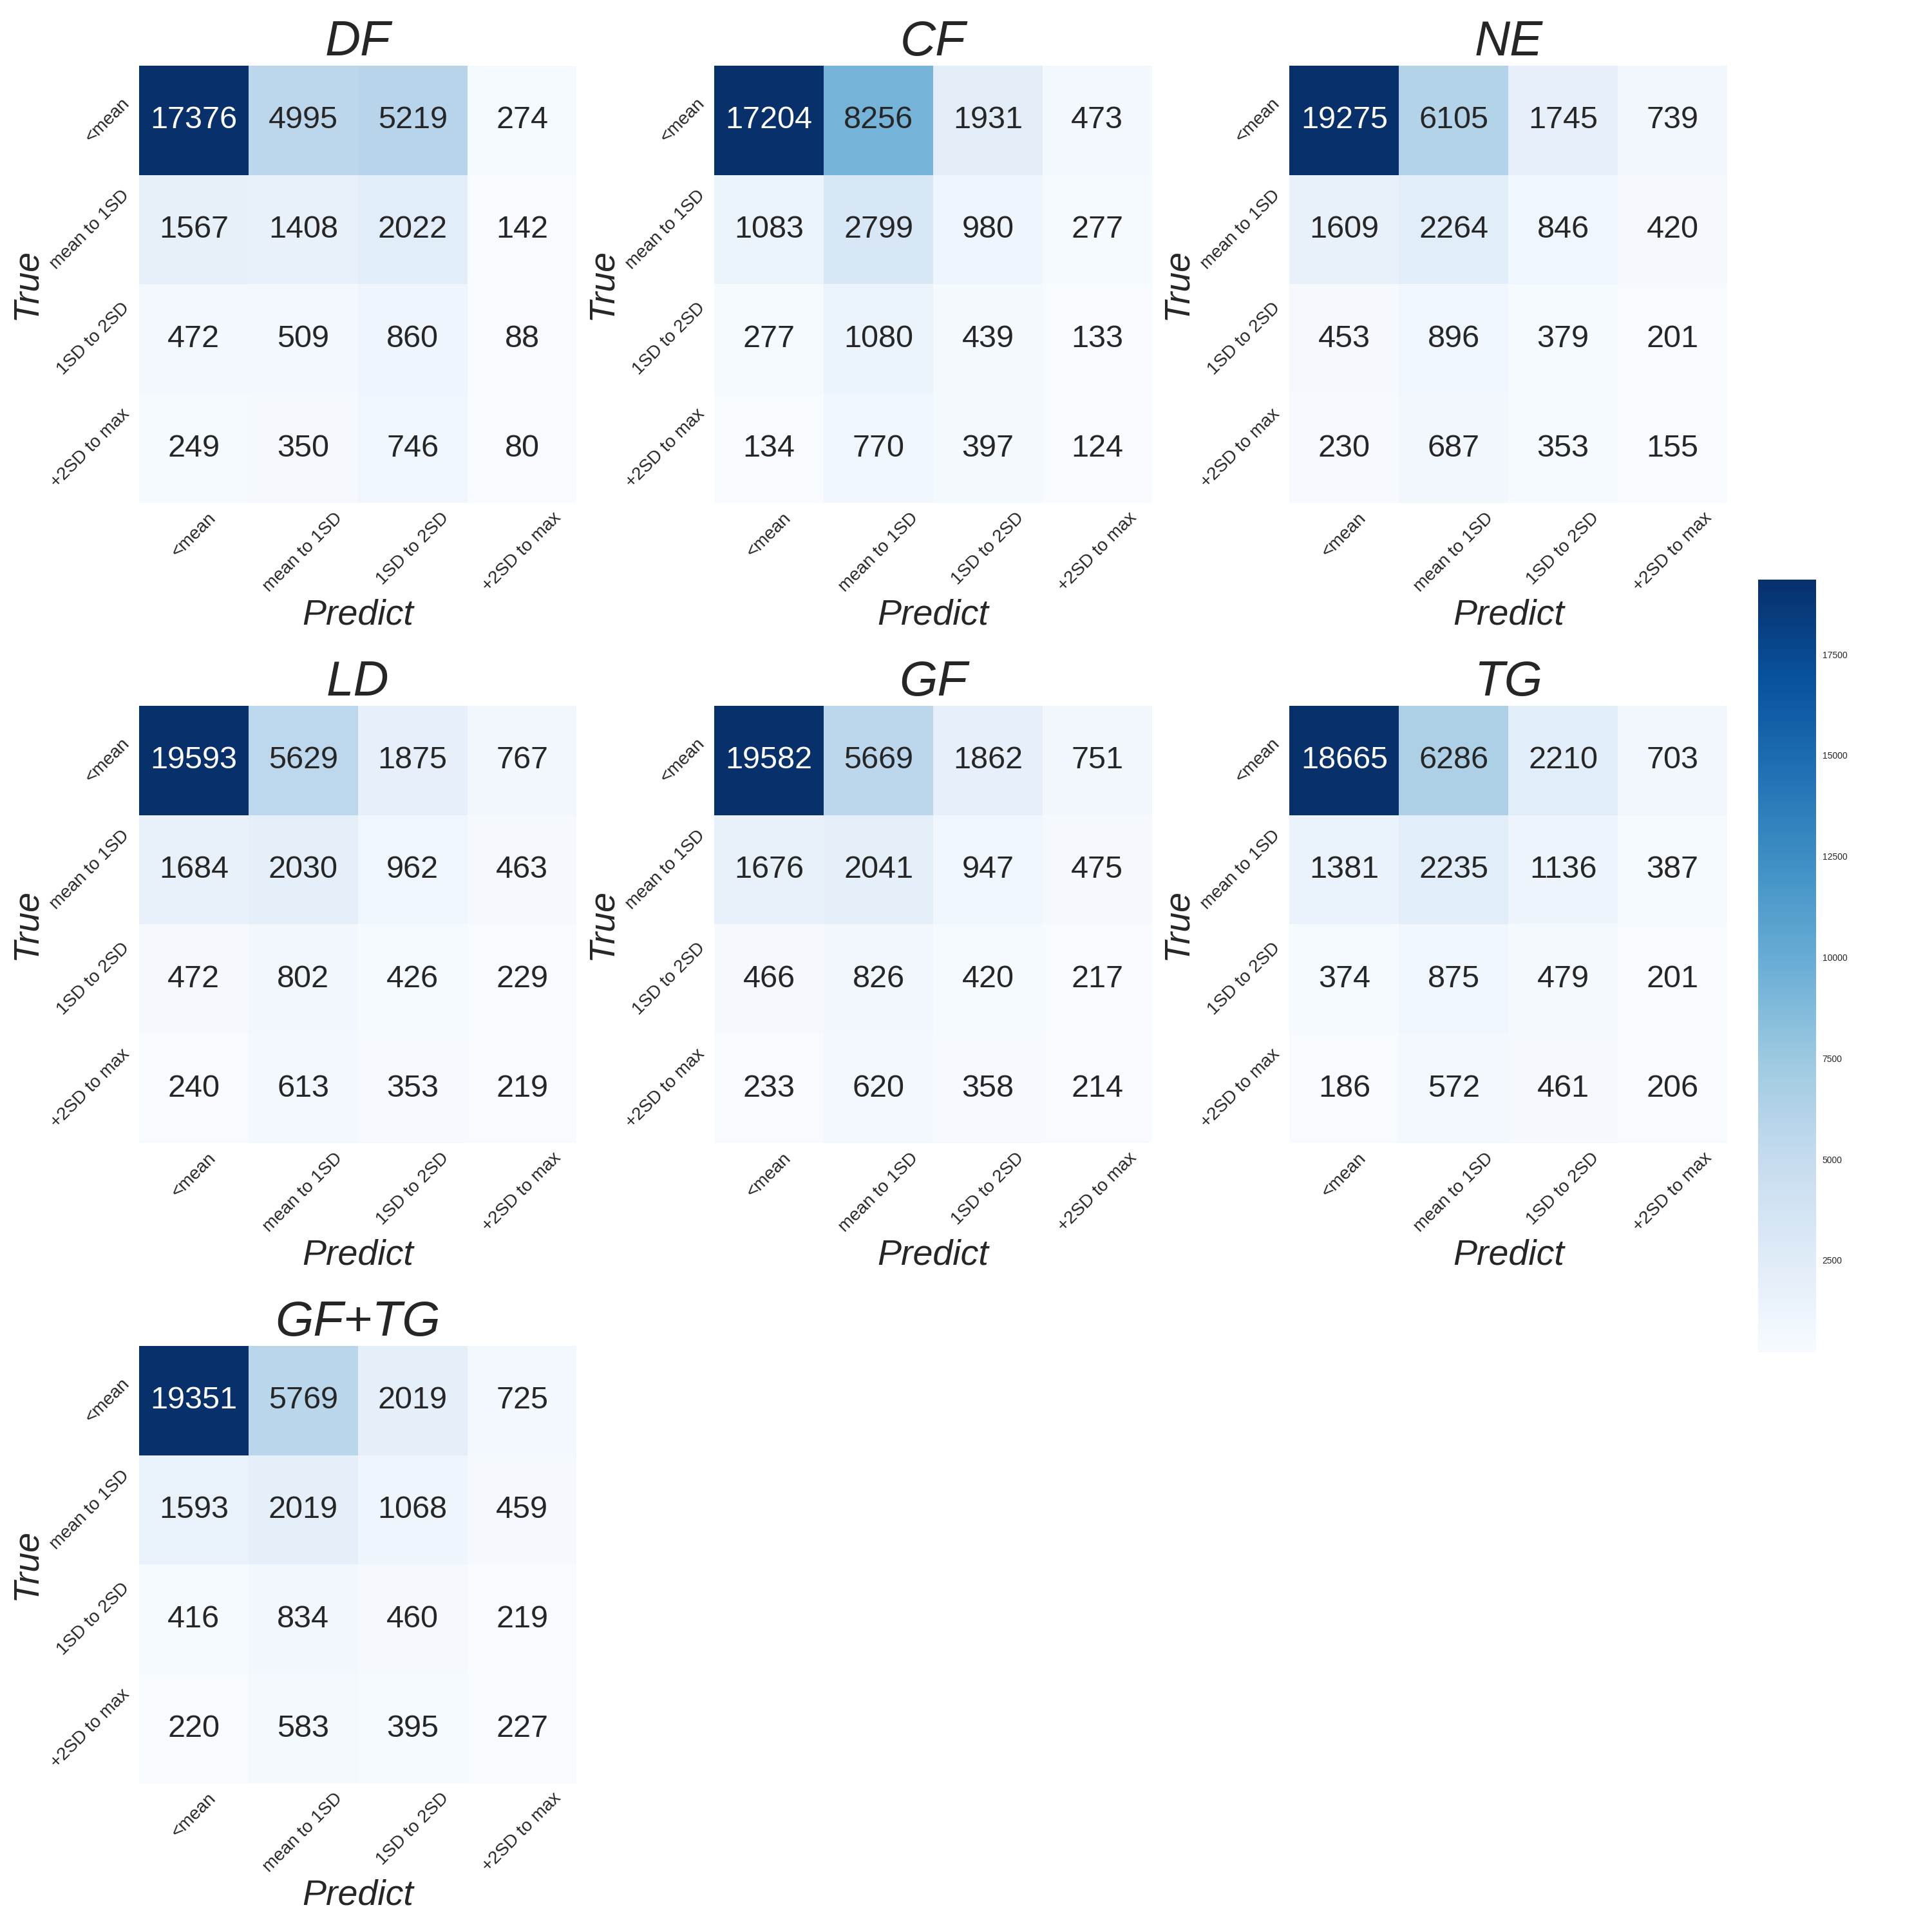
\includegraphics[scale=0.16]{./non-crime-no-timeseries-fig/non_crime_no_timeseries_four_cm.png}
  \caption{4カテゴリーの混同行列}
  \label{fig:non-crime-no-timeseries-4cm}
\end{figure}

\begin{figure}
  \centering % 図を中央寄せにする
  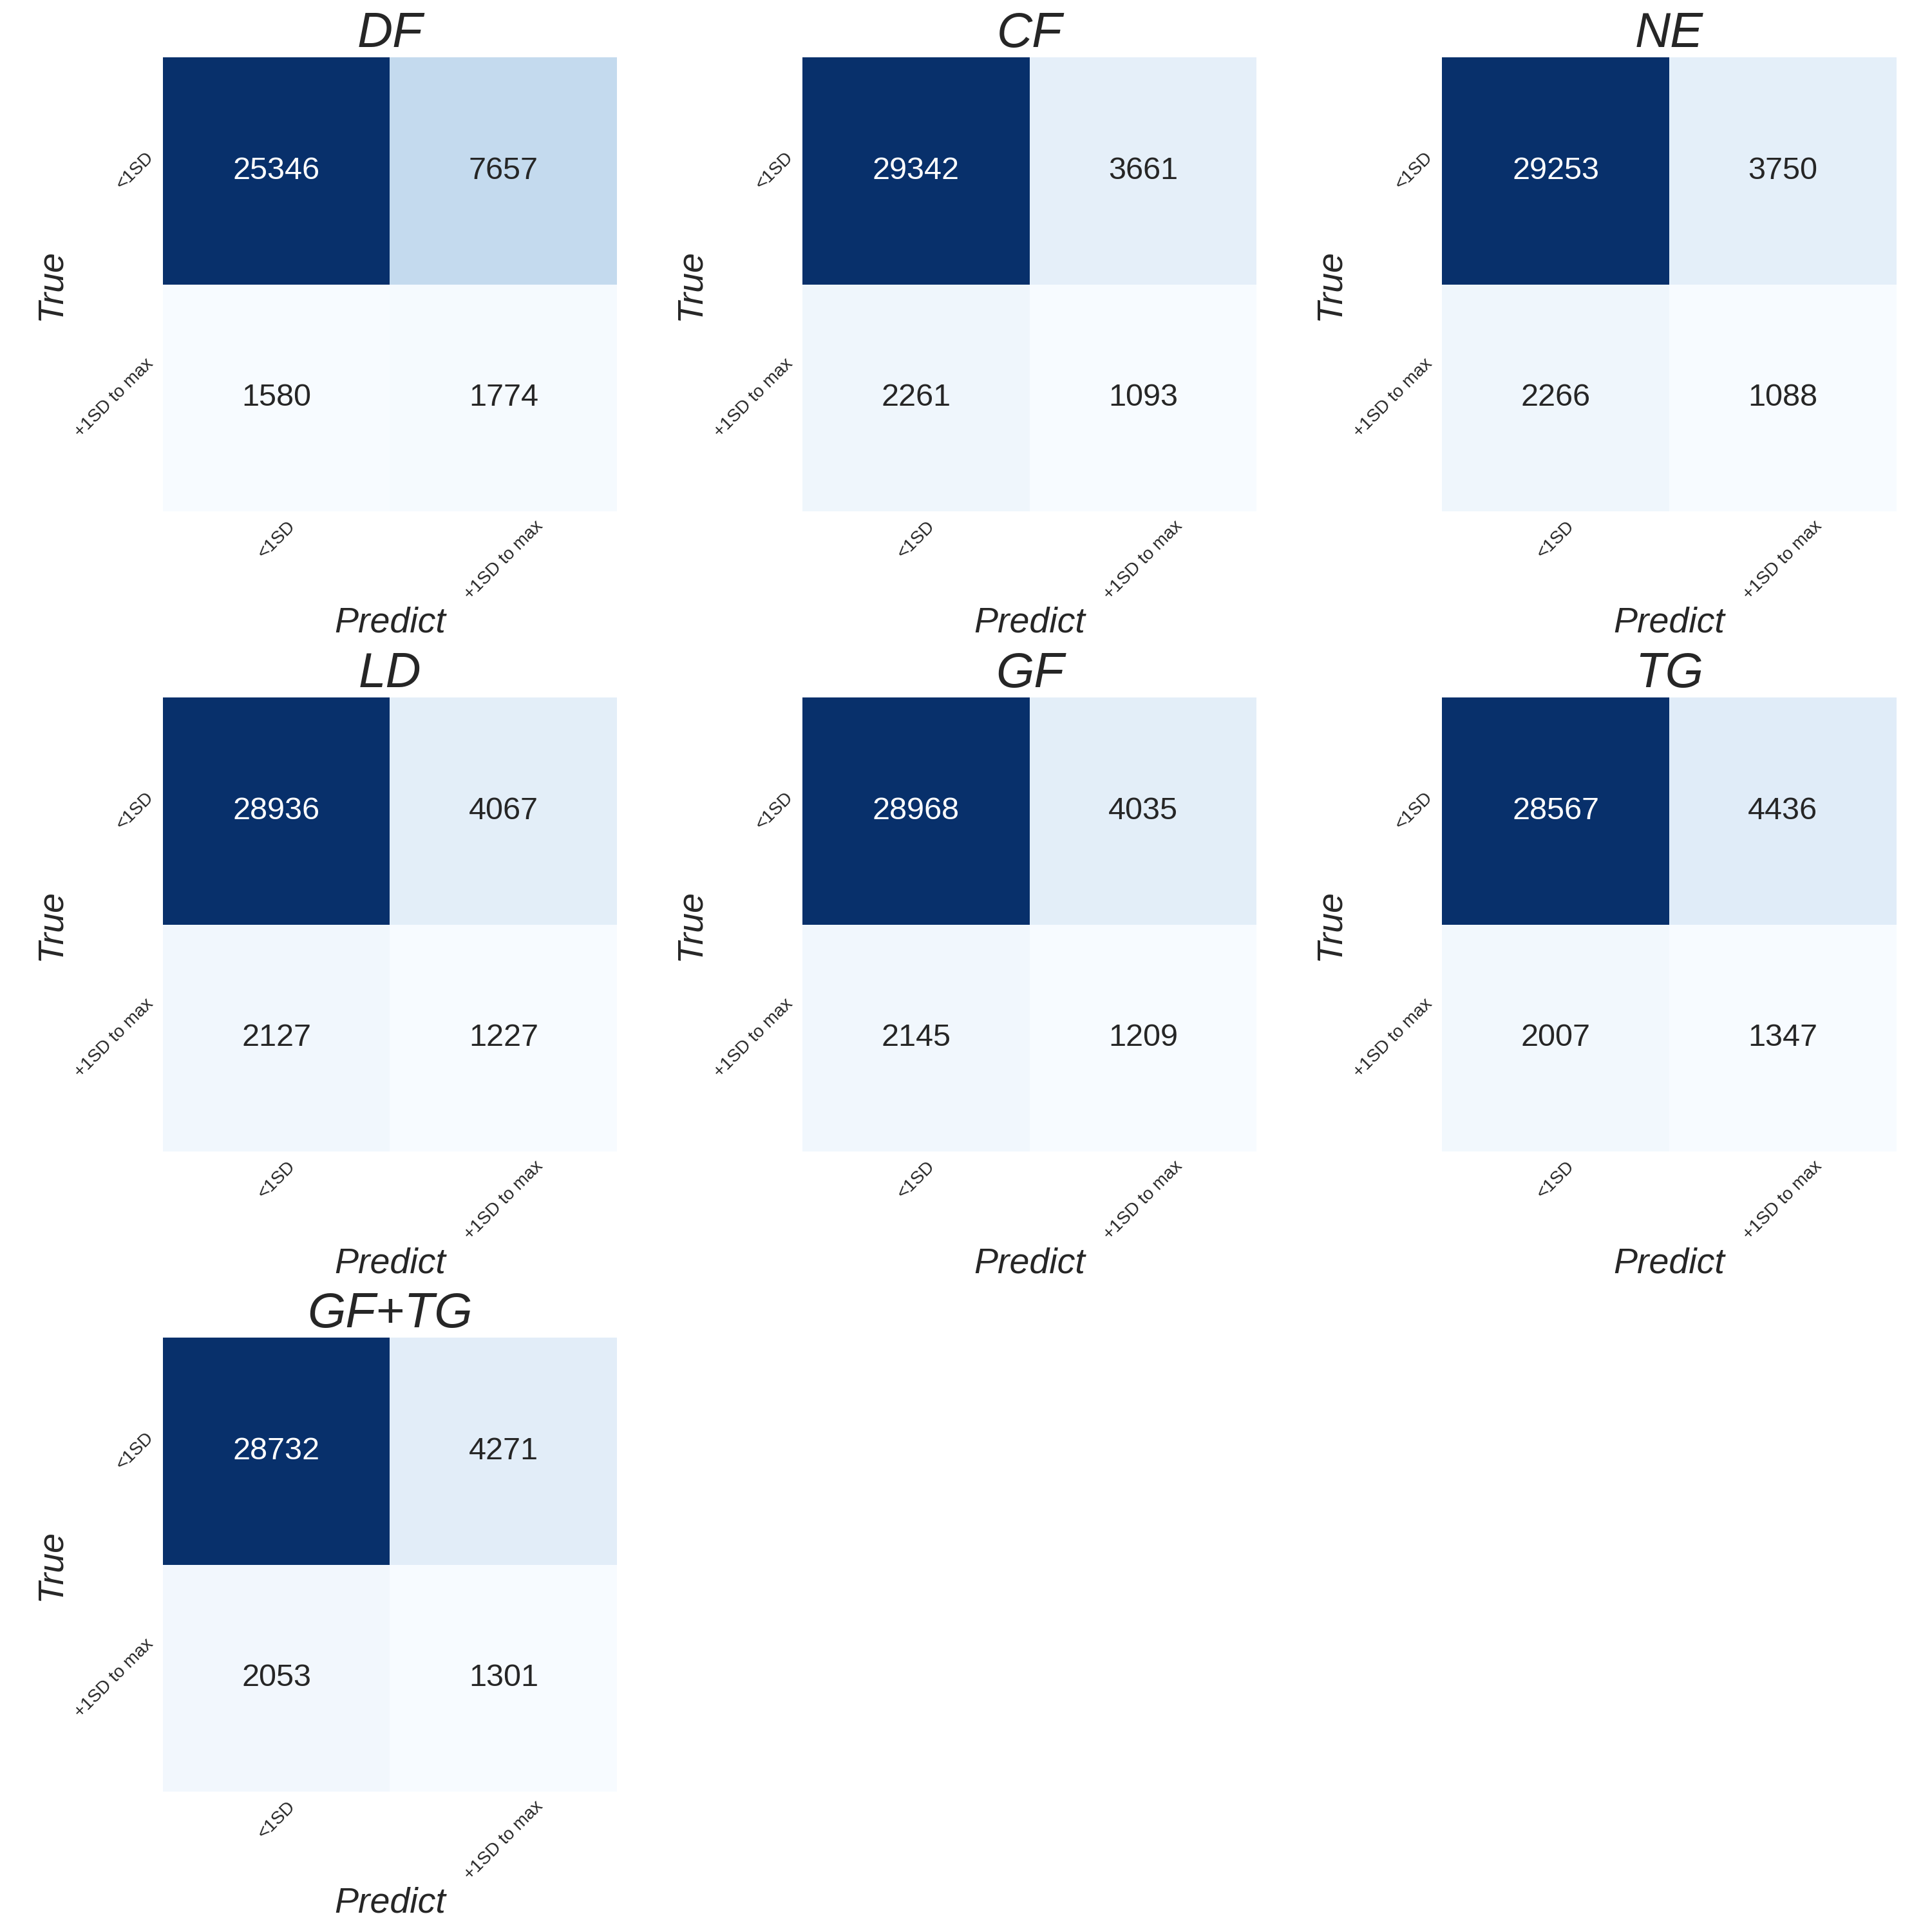
\includegraphics[scale=0.16]{./non-crime-no-timeseries-fig/non_crime_no_timeseries_two_cm.png}
  \caption{2カテゴリーの混同行列}
  \label{fig:non-crime-no-timeseries-2cm}
\end{figure}
% ---------------------------------
% FNFPplot
% ---------------------------------
\begin{figure}
  \centering % 図を中央寄せにする
  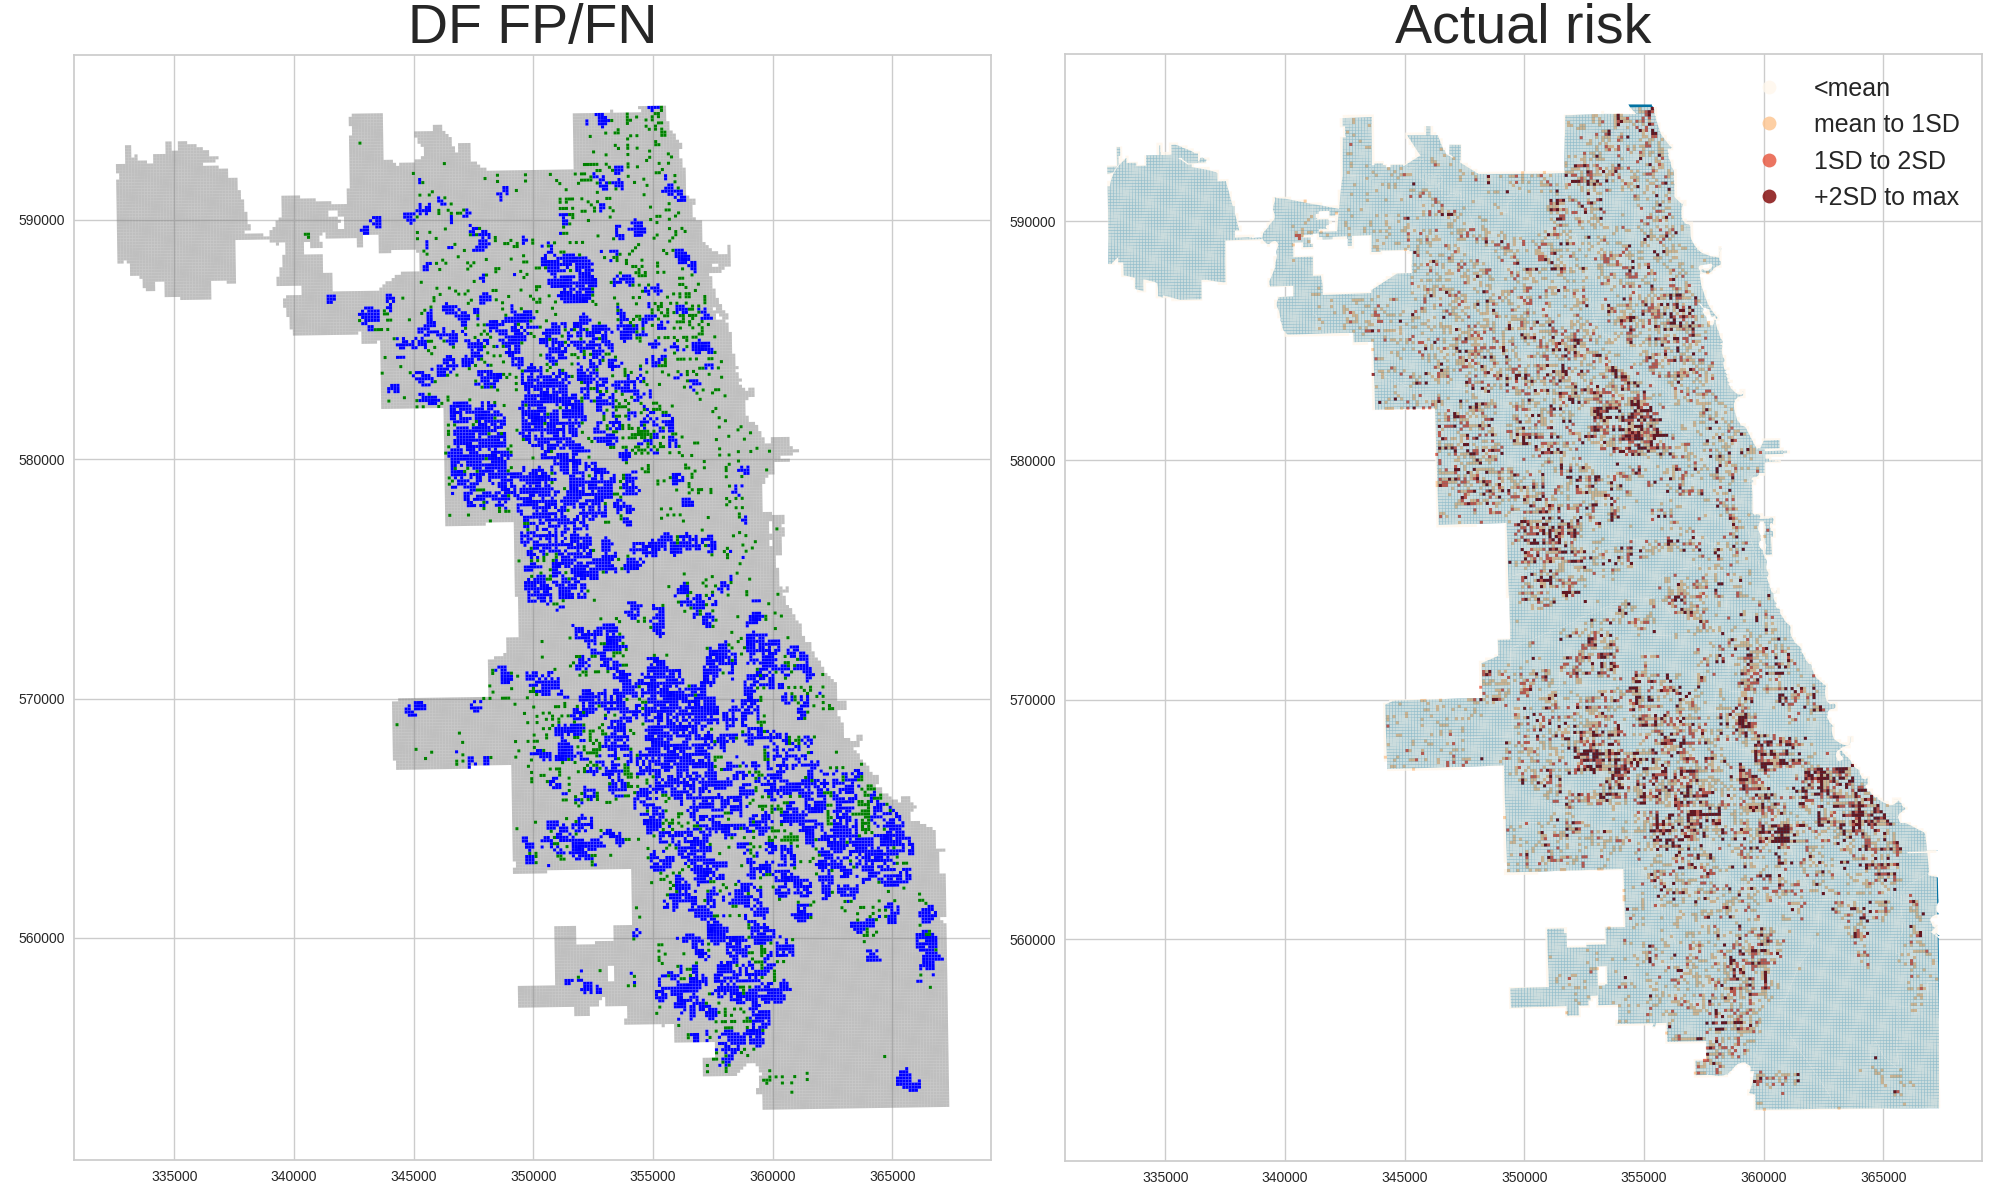
\includegraphics[scale=0.25]{./non-crime-no-timeseries-fig/DF_fnp.png}
  \caption{左:DFのFPFN 右:実際のリスクマップ}
  \label{fig:non-crime-no-timeseries-df-fnp}
\end{figure}

\begin{figure}
  \centering % 図を中央寄せにする
  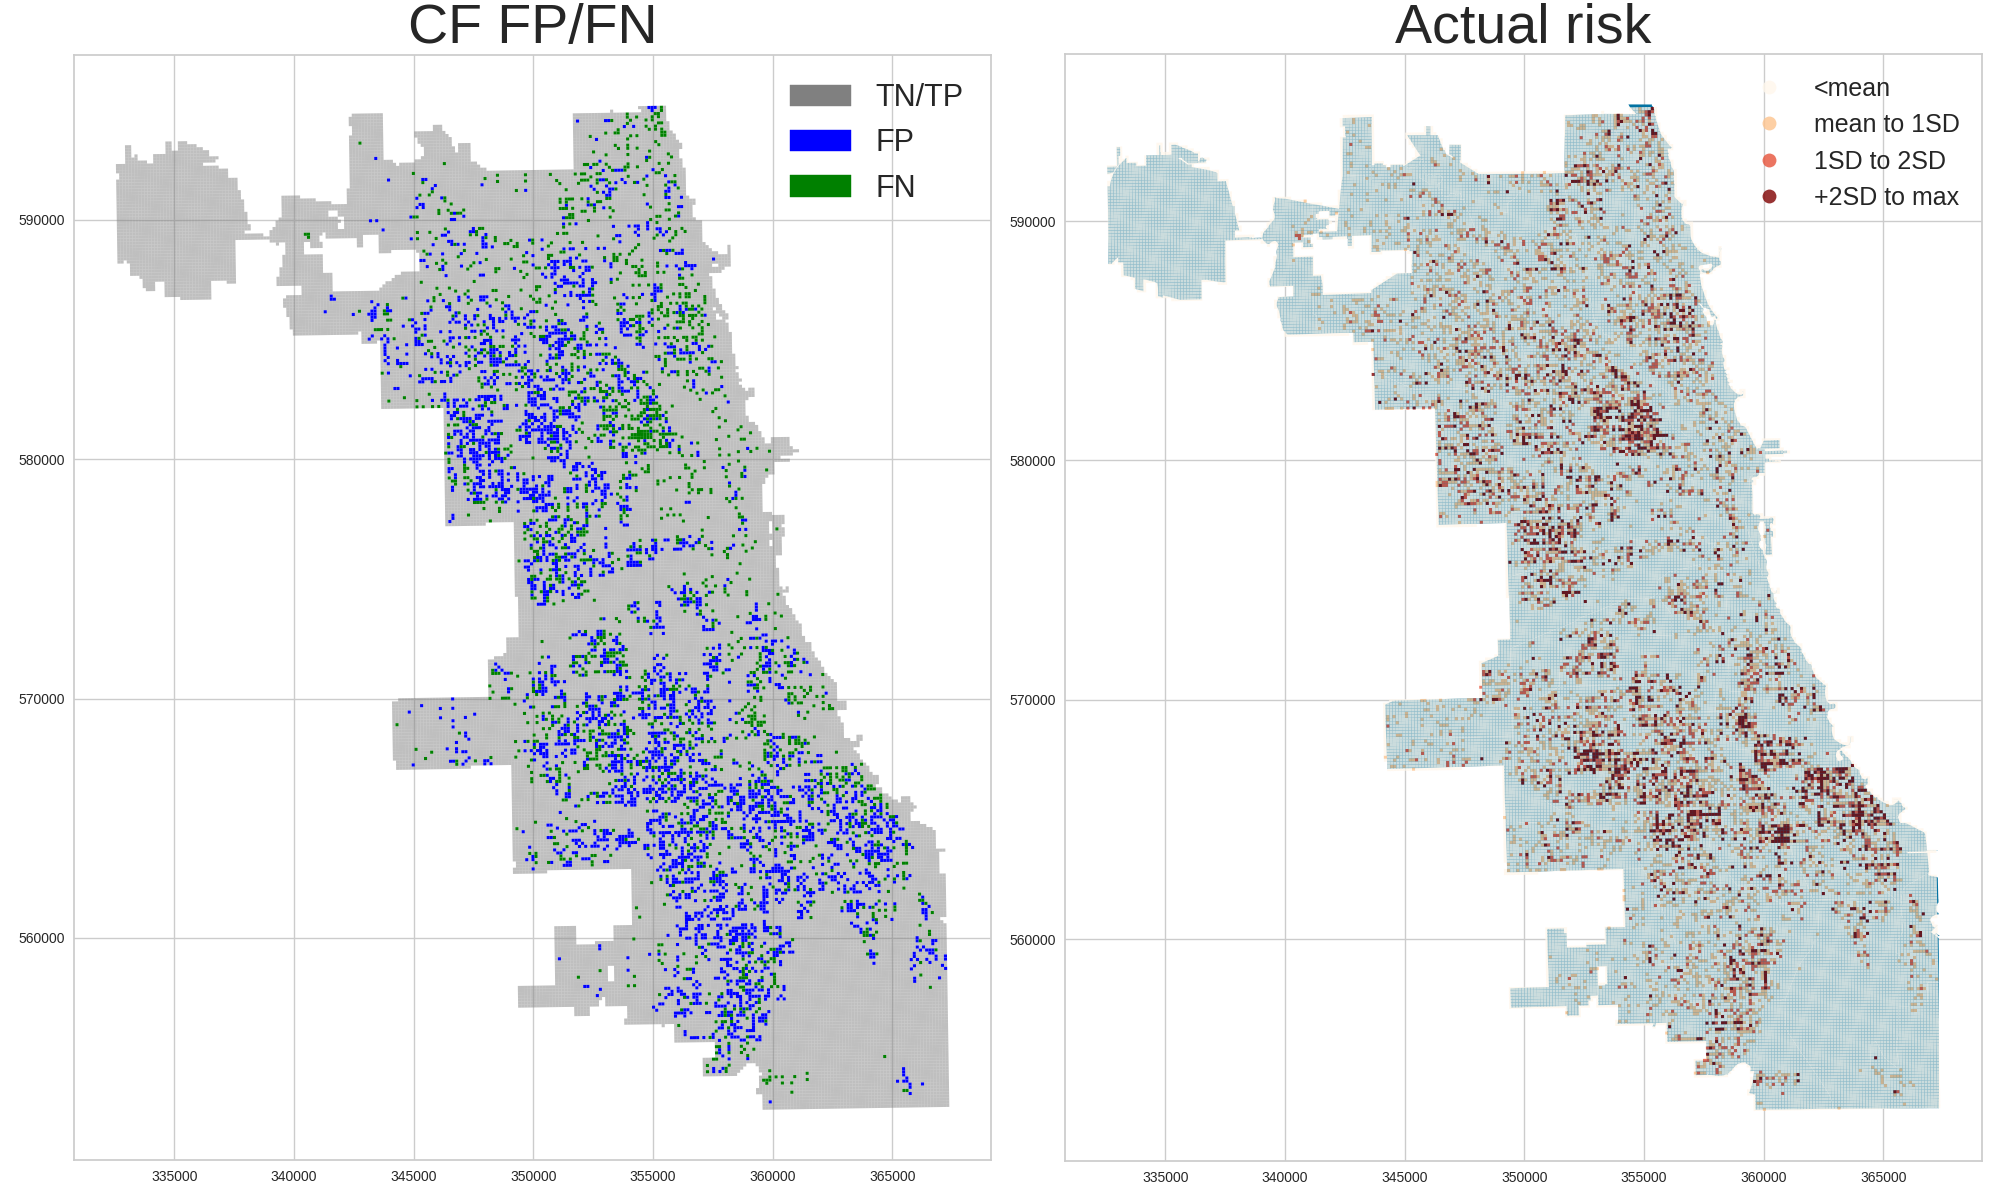
\includegraphics[scale=0.25]{./non-crime-no-timeseries-fig/CF_fnp.png}
  \caption{左:CFのFPFN 右:実際のリスクマップ}
  \label{fig:non-crime-no-timeseries-cf-fnp}
\end{figure}

\begin{figure}
  \centering % 図を中央寄せにする
  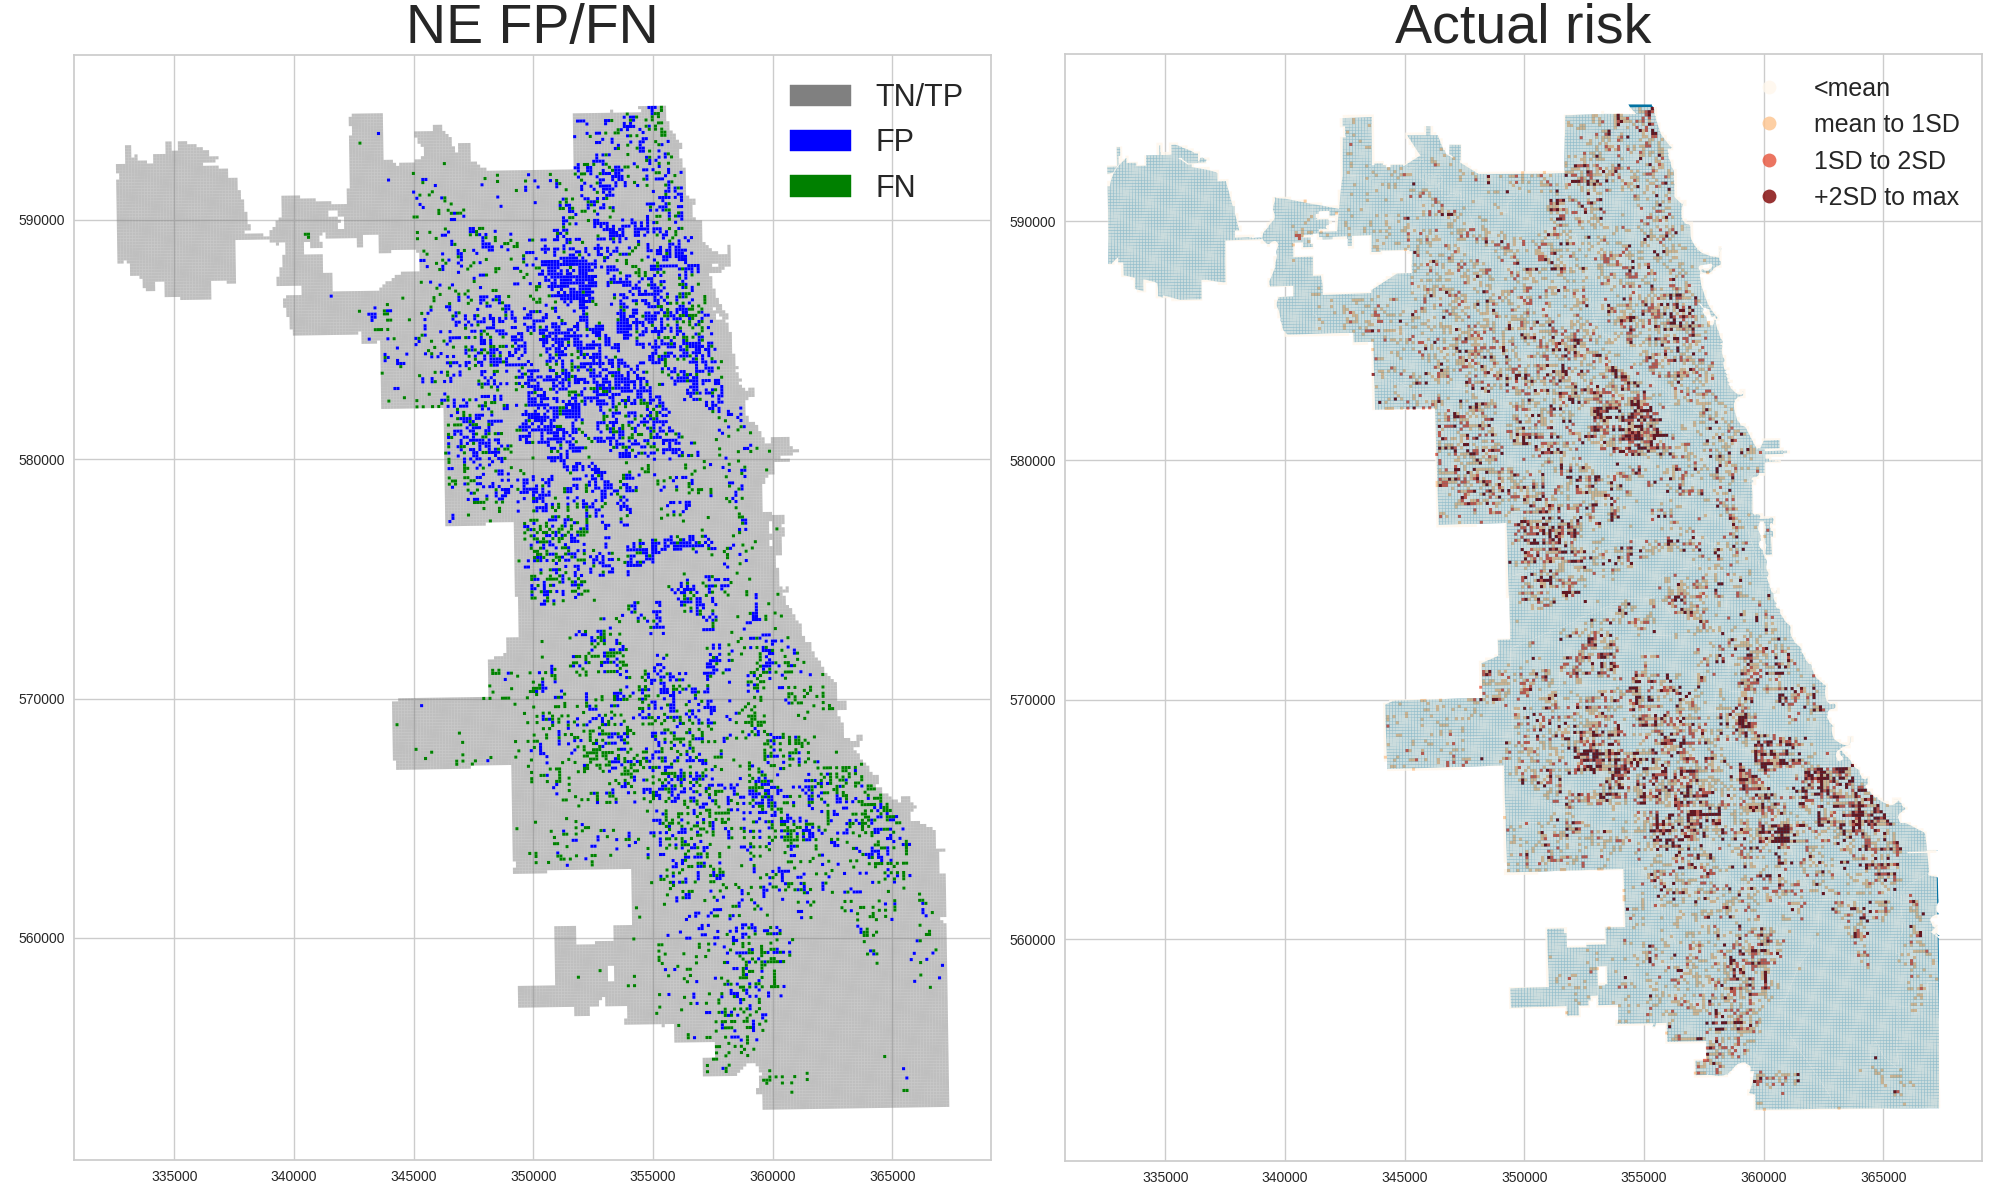
\includegraphics[scale=0.25]{./non-crime-no-timeseries-fig/NE_fnp.png}
  \caption{左:NEのFPFN 右:実際のリスクマップ}
  \label{fig:non-crime-no-timeseries-ne-fnp}
\end{figure}

\begin{figure}
  \centering % 図を中央寄せにする
  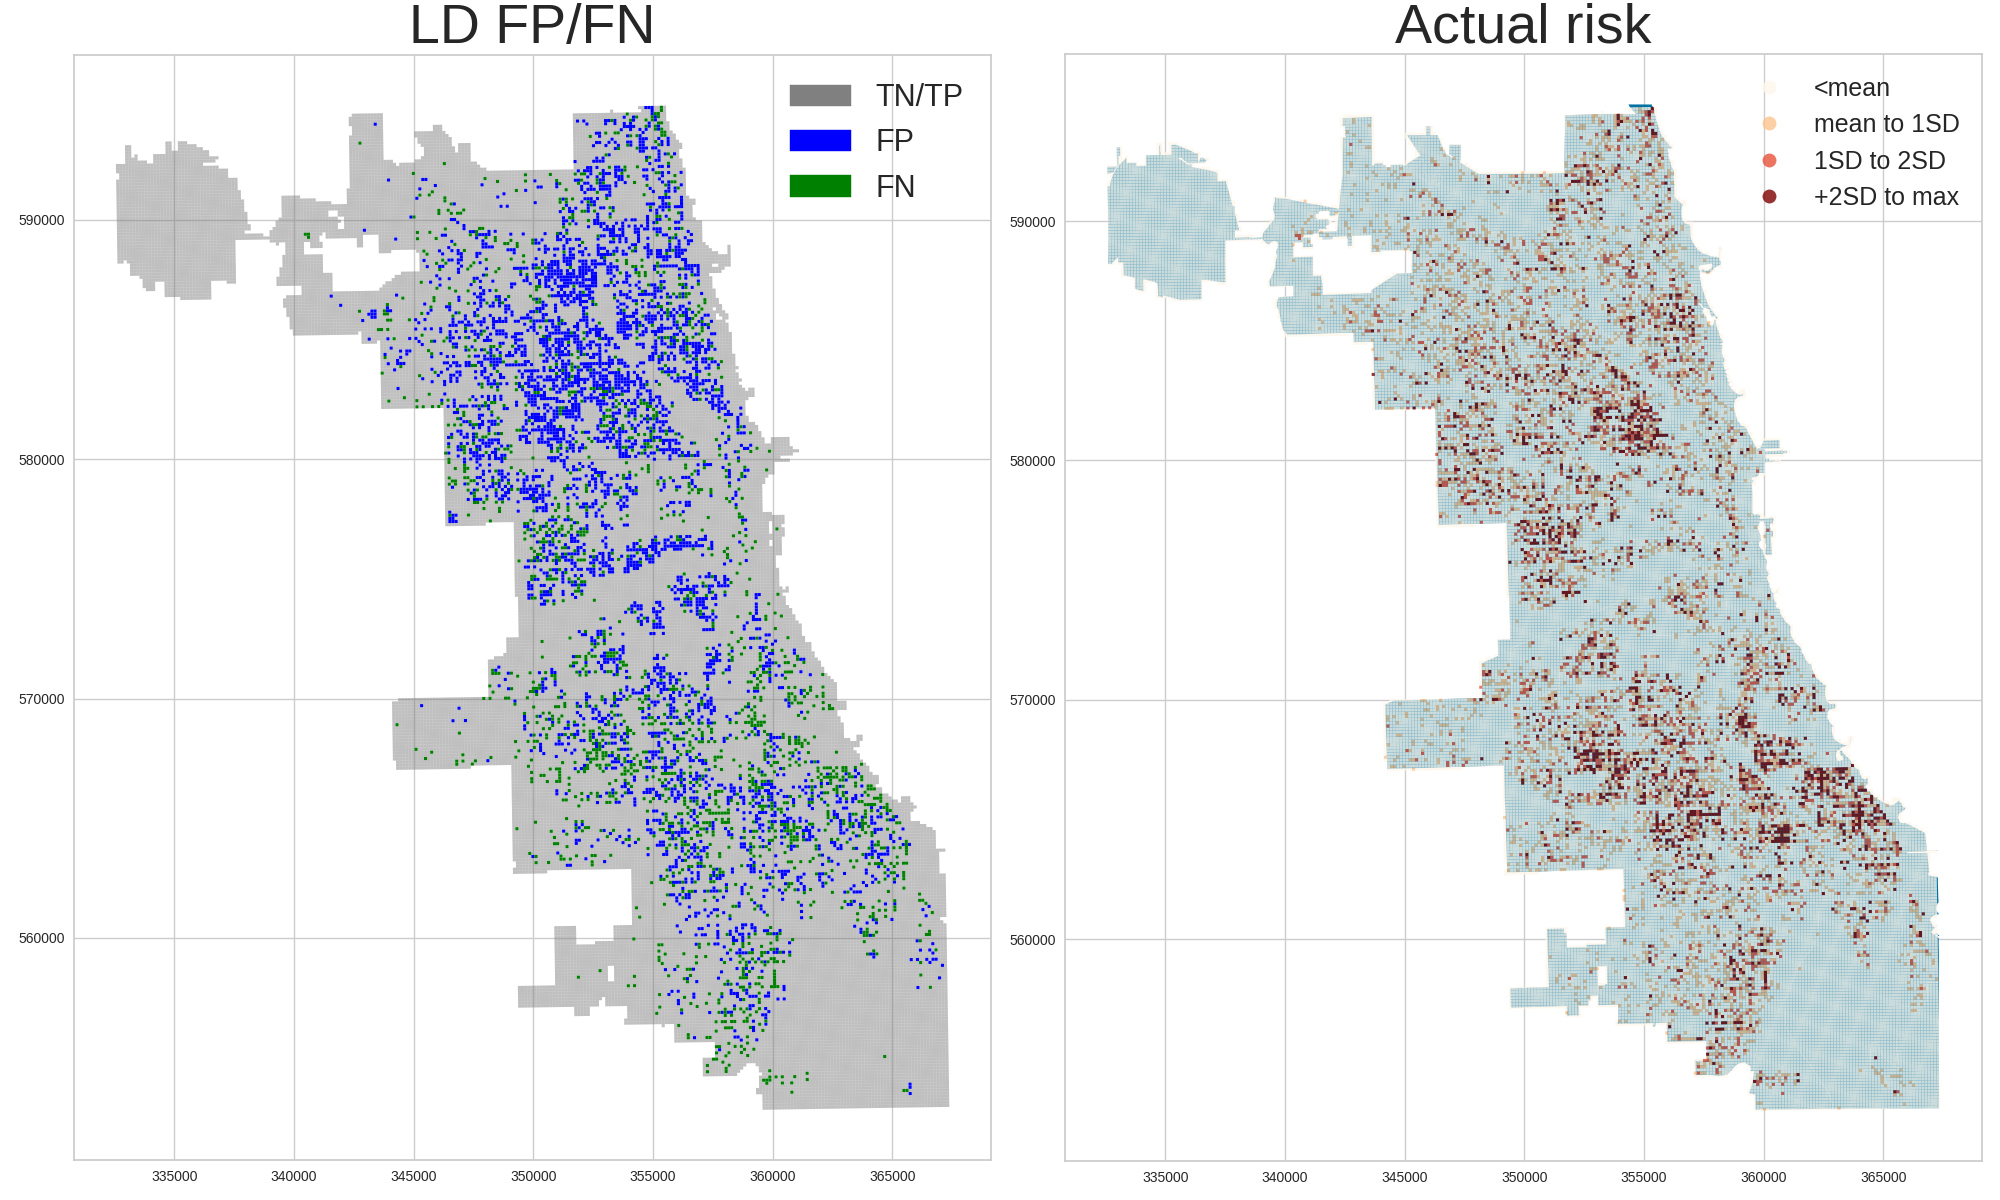
\includegraphics[scale=0.25]{./non-crime-no-timeseries-fig/LD_fnp.png}
  \caption{左:LDのFPFN 右:実際のリスクマップ}
  \label{fig:non-crime-no-timeseries-ld-fnp}
\end{figure}

\begin{figure}
  \centering % 図を中央寄せにする
  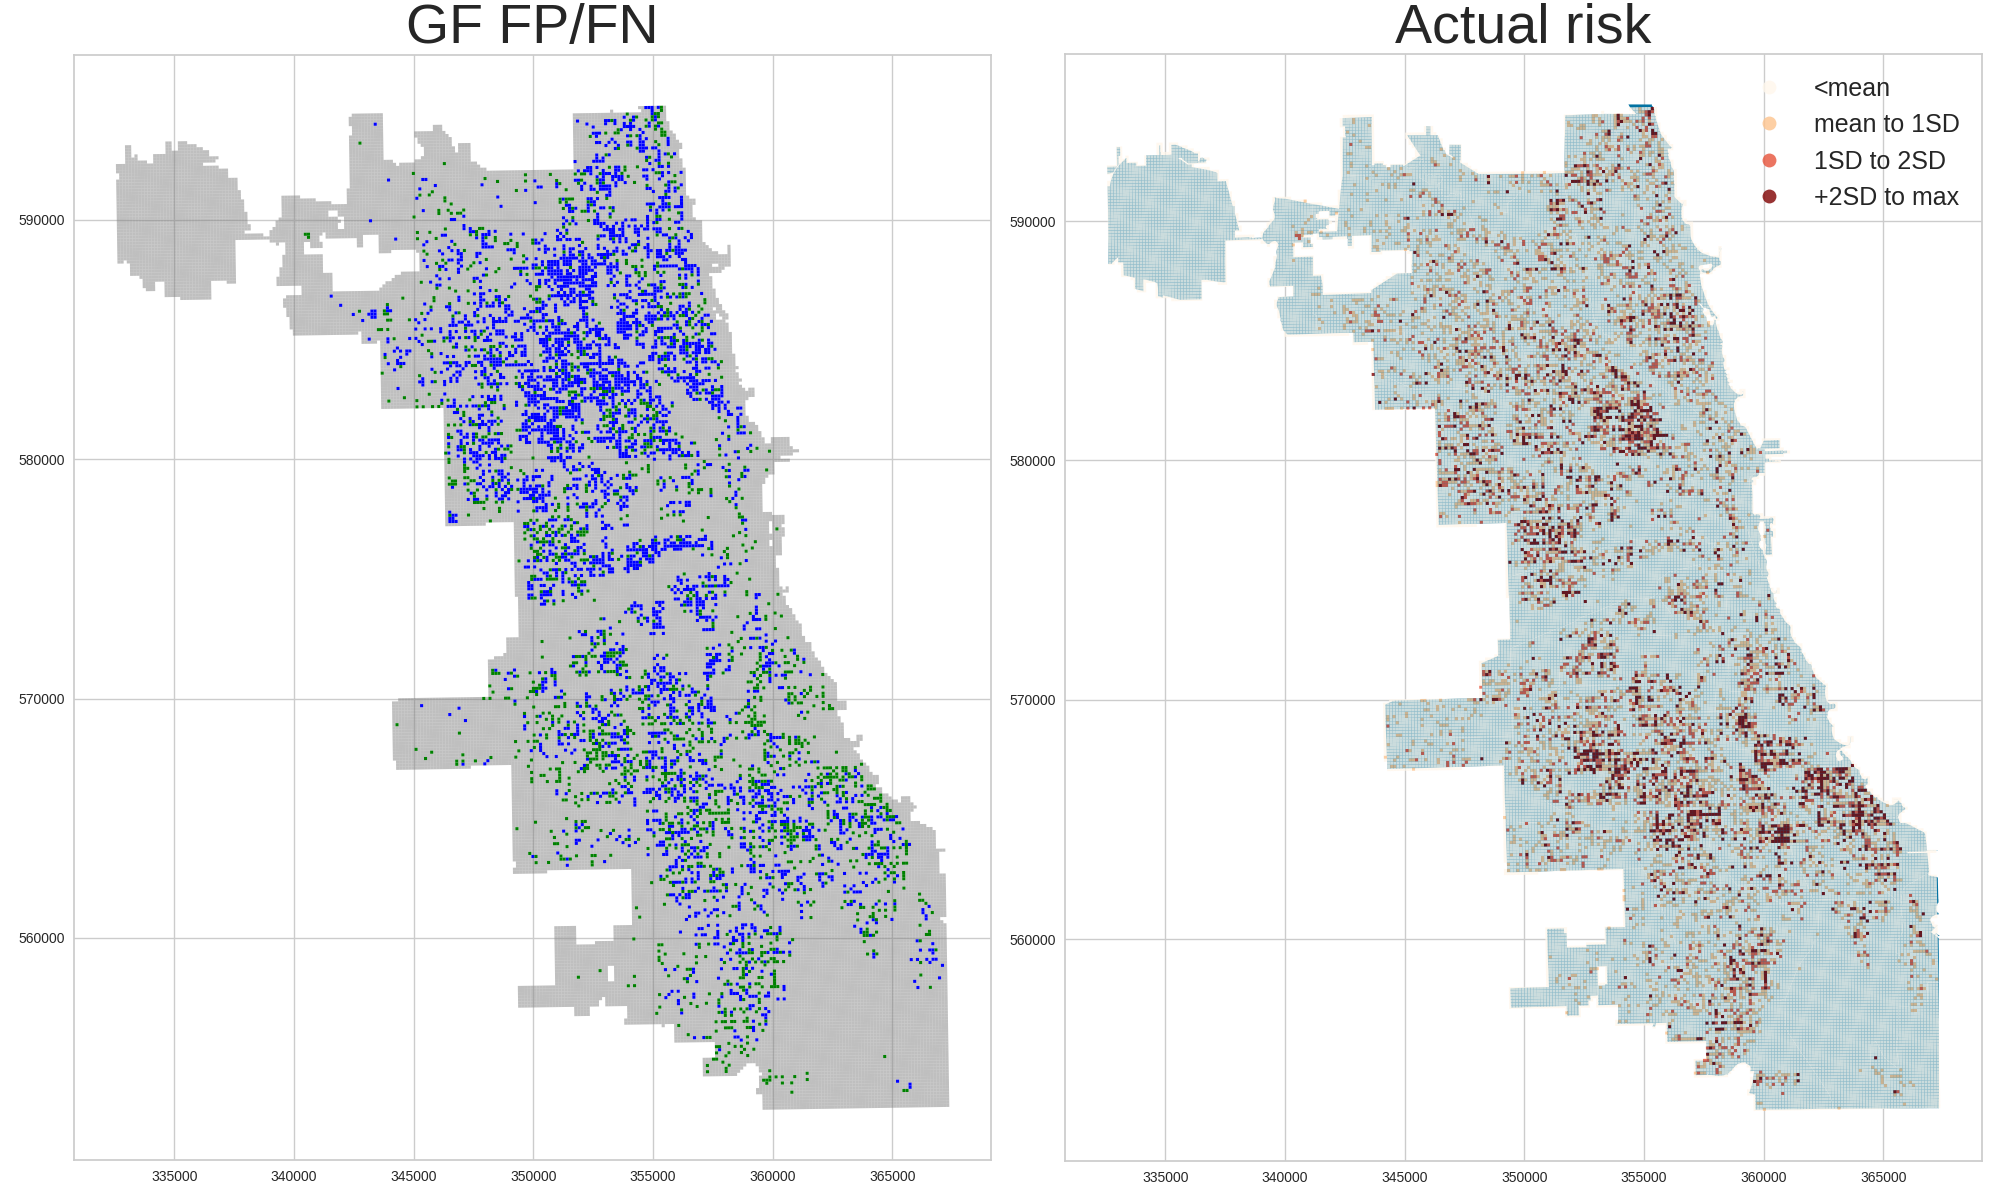
\includegraphics[scale=0.25]{./non-crime-no-timeseries-fig/GF_fnp.png}
  \caption{左:GFのFPFN 右:実際のリスクマップ}
  \label{fig:non-crime-no-timeseries-gf-fnp}
\end{figure}

\begin{figure}
  \centering % 図を中央寄せにする
  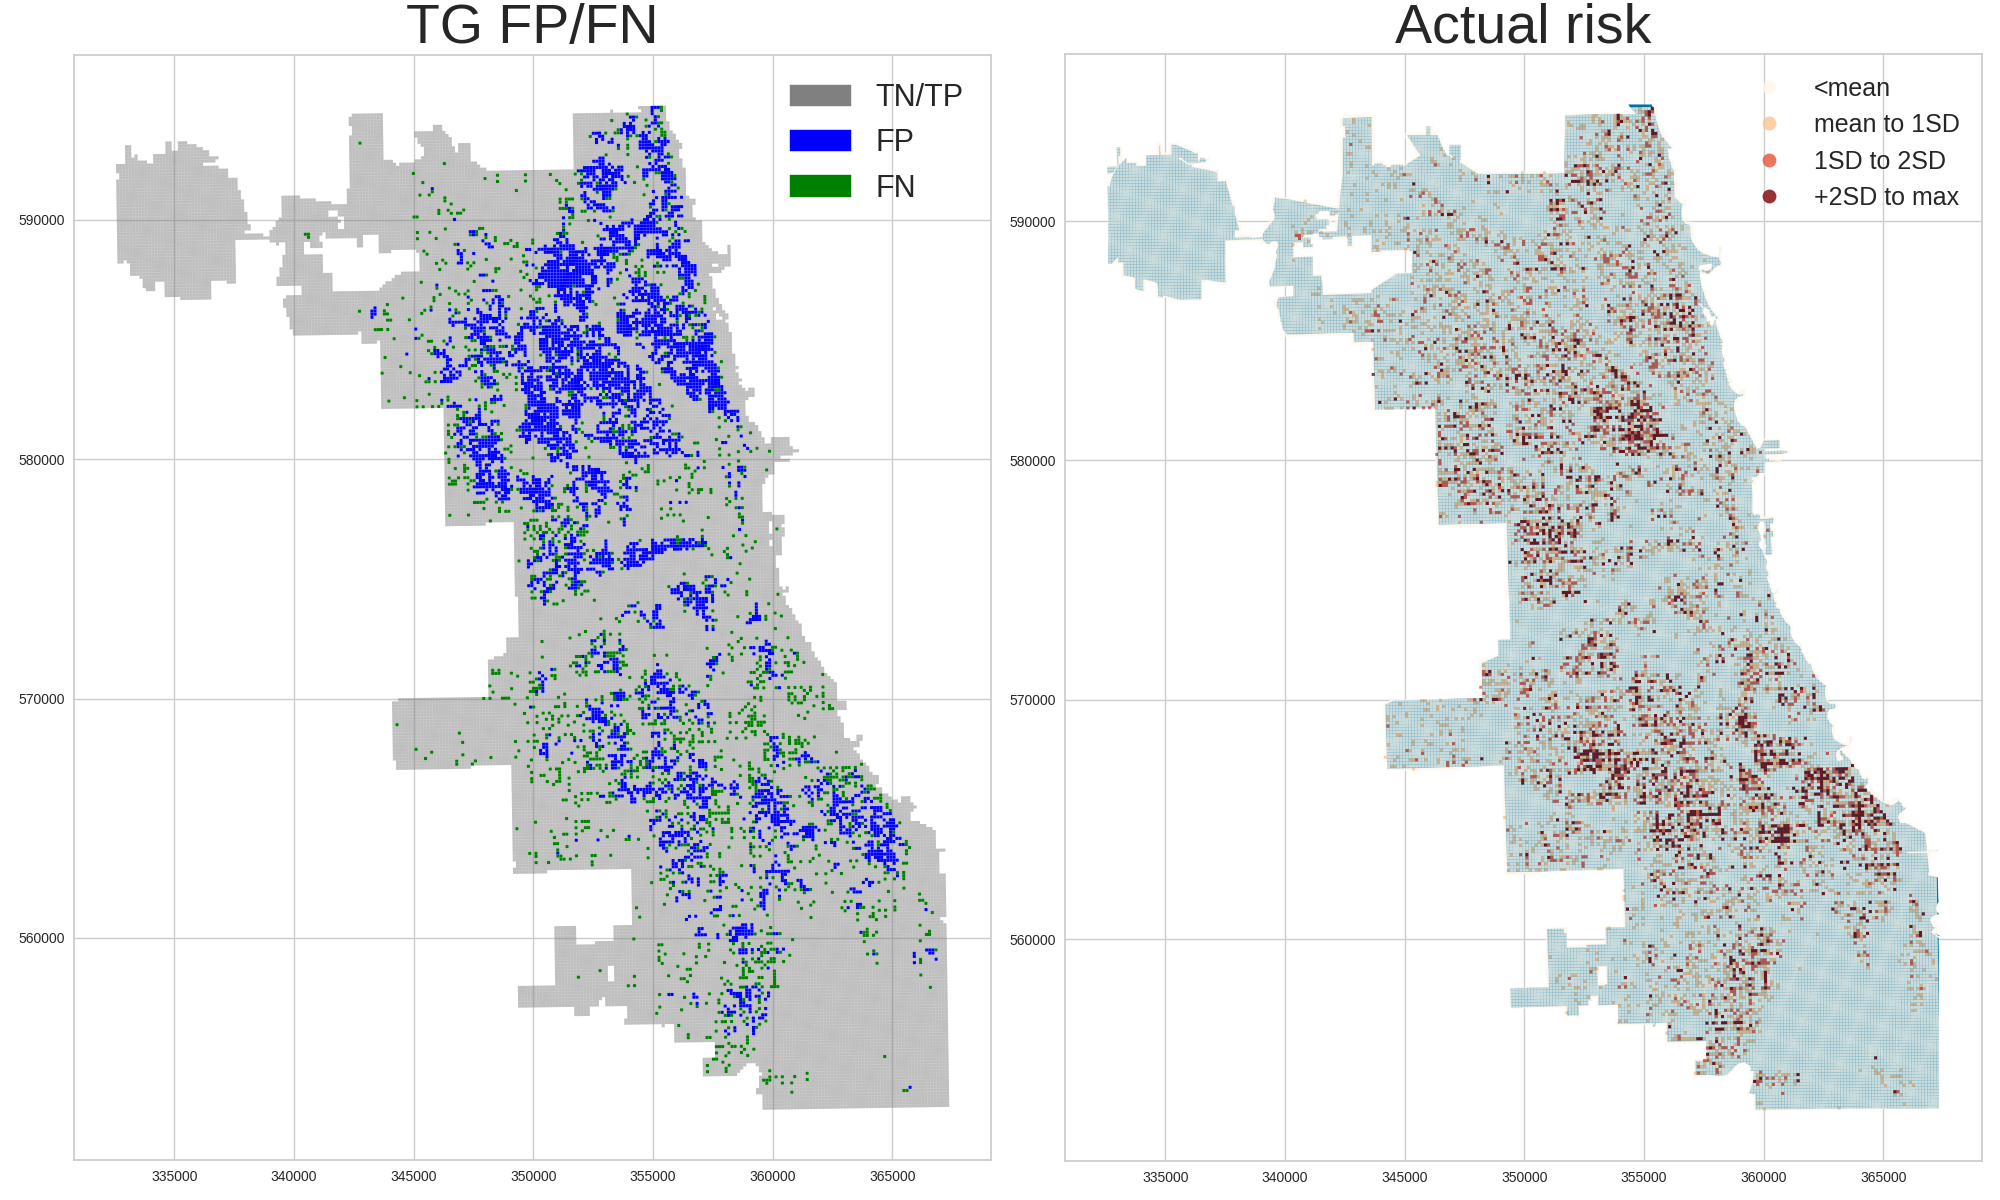
\includegraphics[scale=0.25]{./non-crime-no-timeseries-fig/TG_fnp.png}
  \caption{左:TGのFPFN 右:実際のリスクマップ}
  \label{fig:non-crime-no-timeseries-tg-fnp}
\end{figure}

\begin{figure}
  \centering % 図を中央寄せにする
  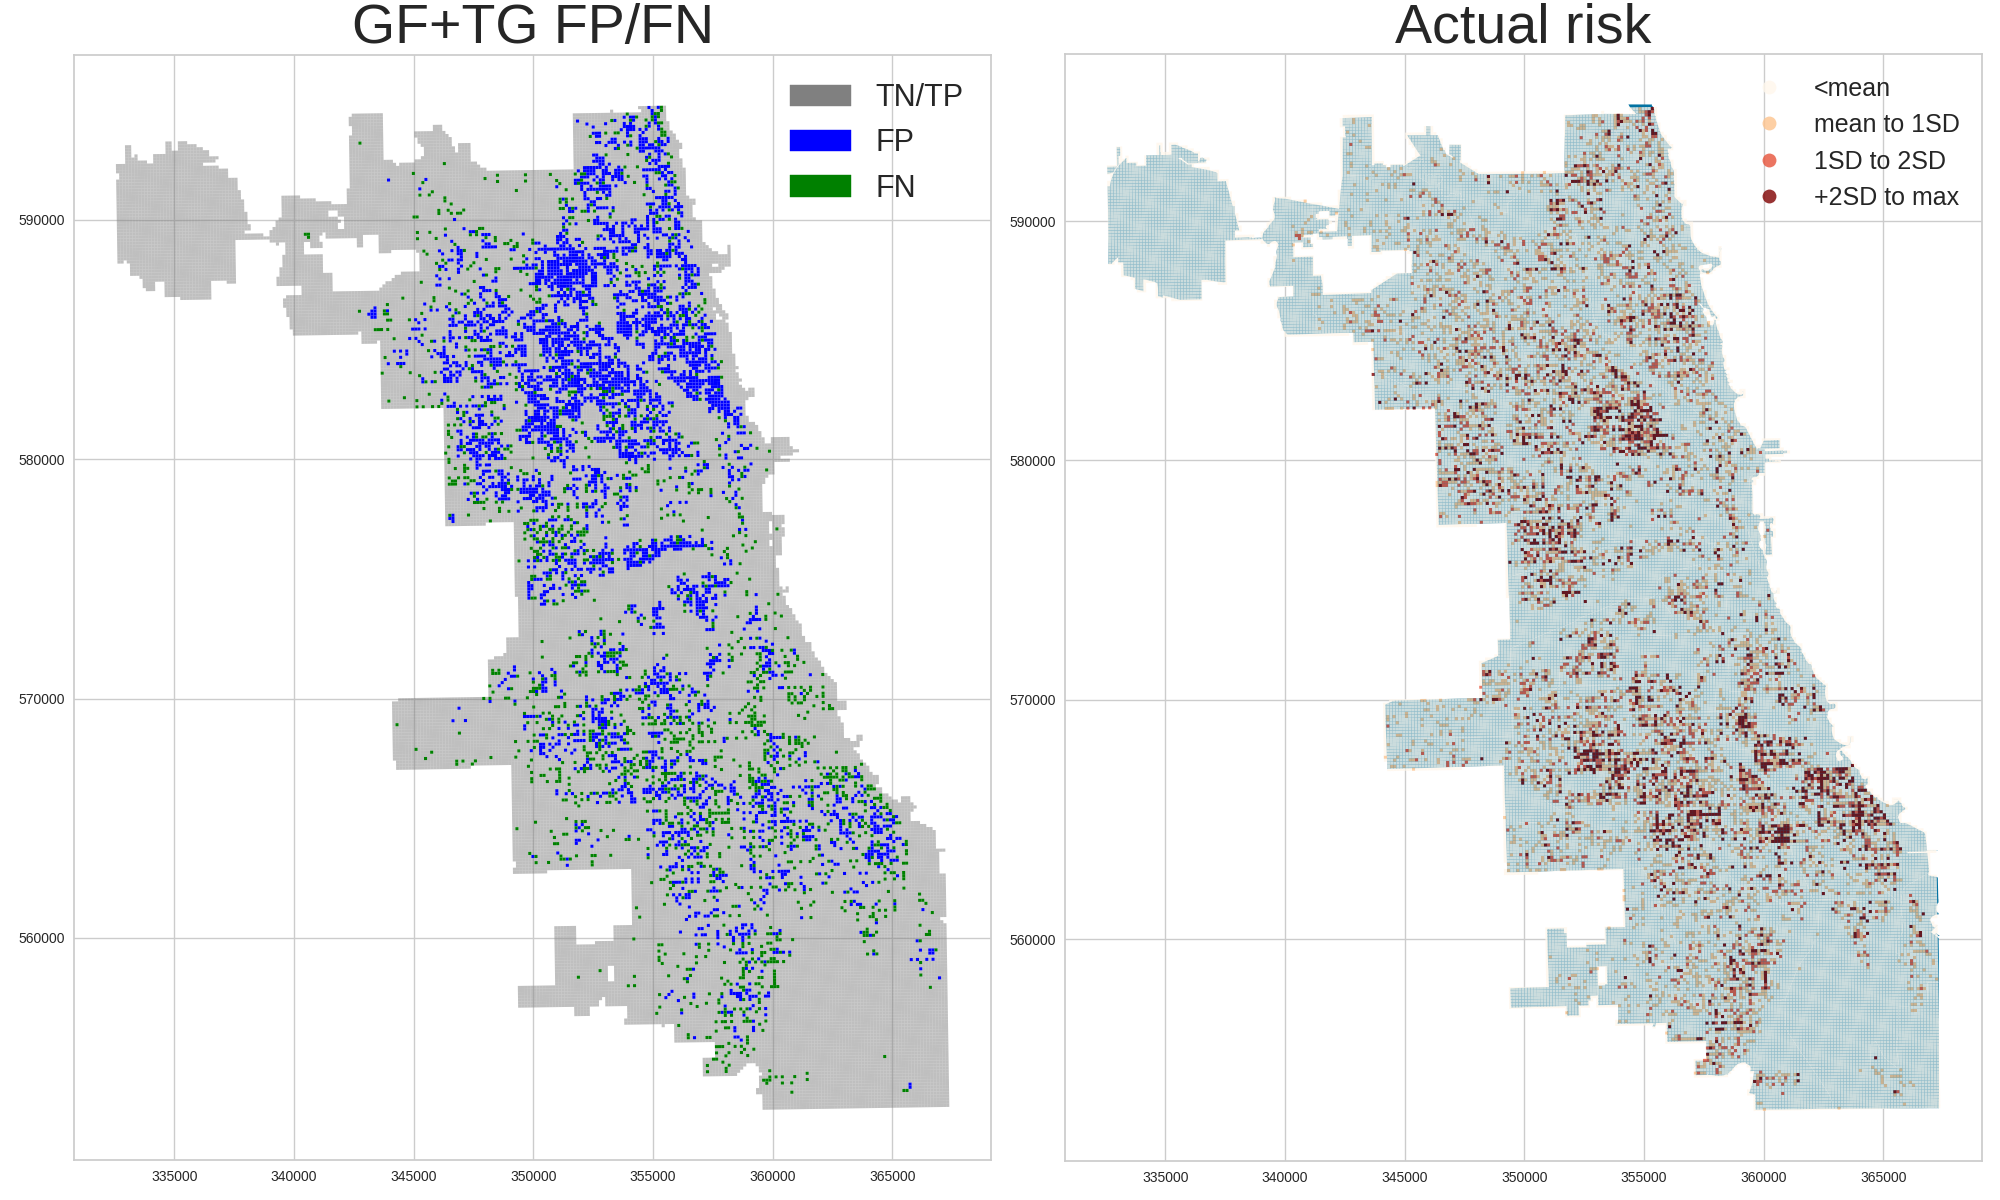
\includegraphics[scale=0.25]{./non-crime-no-timeseries-fig/GF+TG_fnp.png}
  \caption{左:GF+TGのFPFN 右:実際のリスクマップ}
  \label{fig:non-crime-no-timeseries-gf-tg-fnp}
\end{figure}
%------------------------------------------
% ROC curve
%------------------------------------------
また,各モデルのROC曲線を図\ref{fig:non-crime-no-timeseries-roc}に示した.

\begin{figure}
  \centering % 図を中央寄せにする
  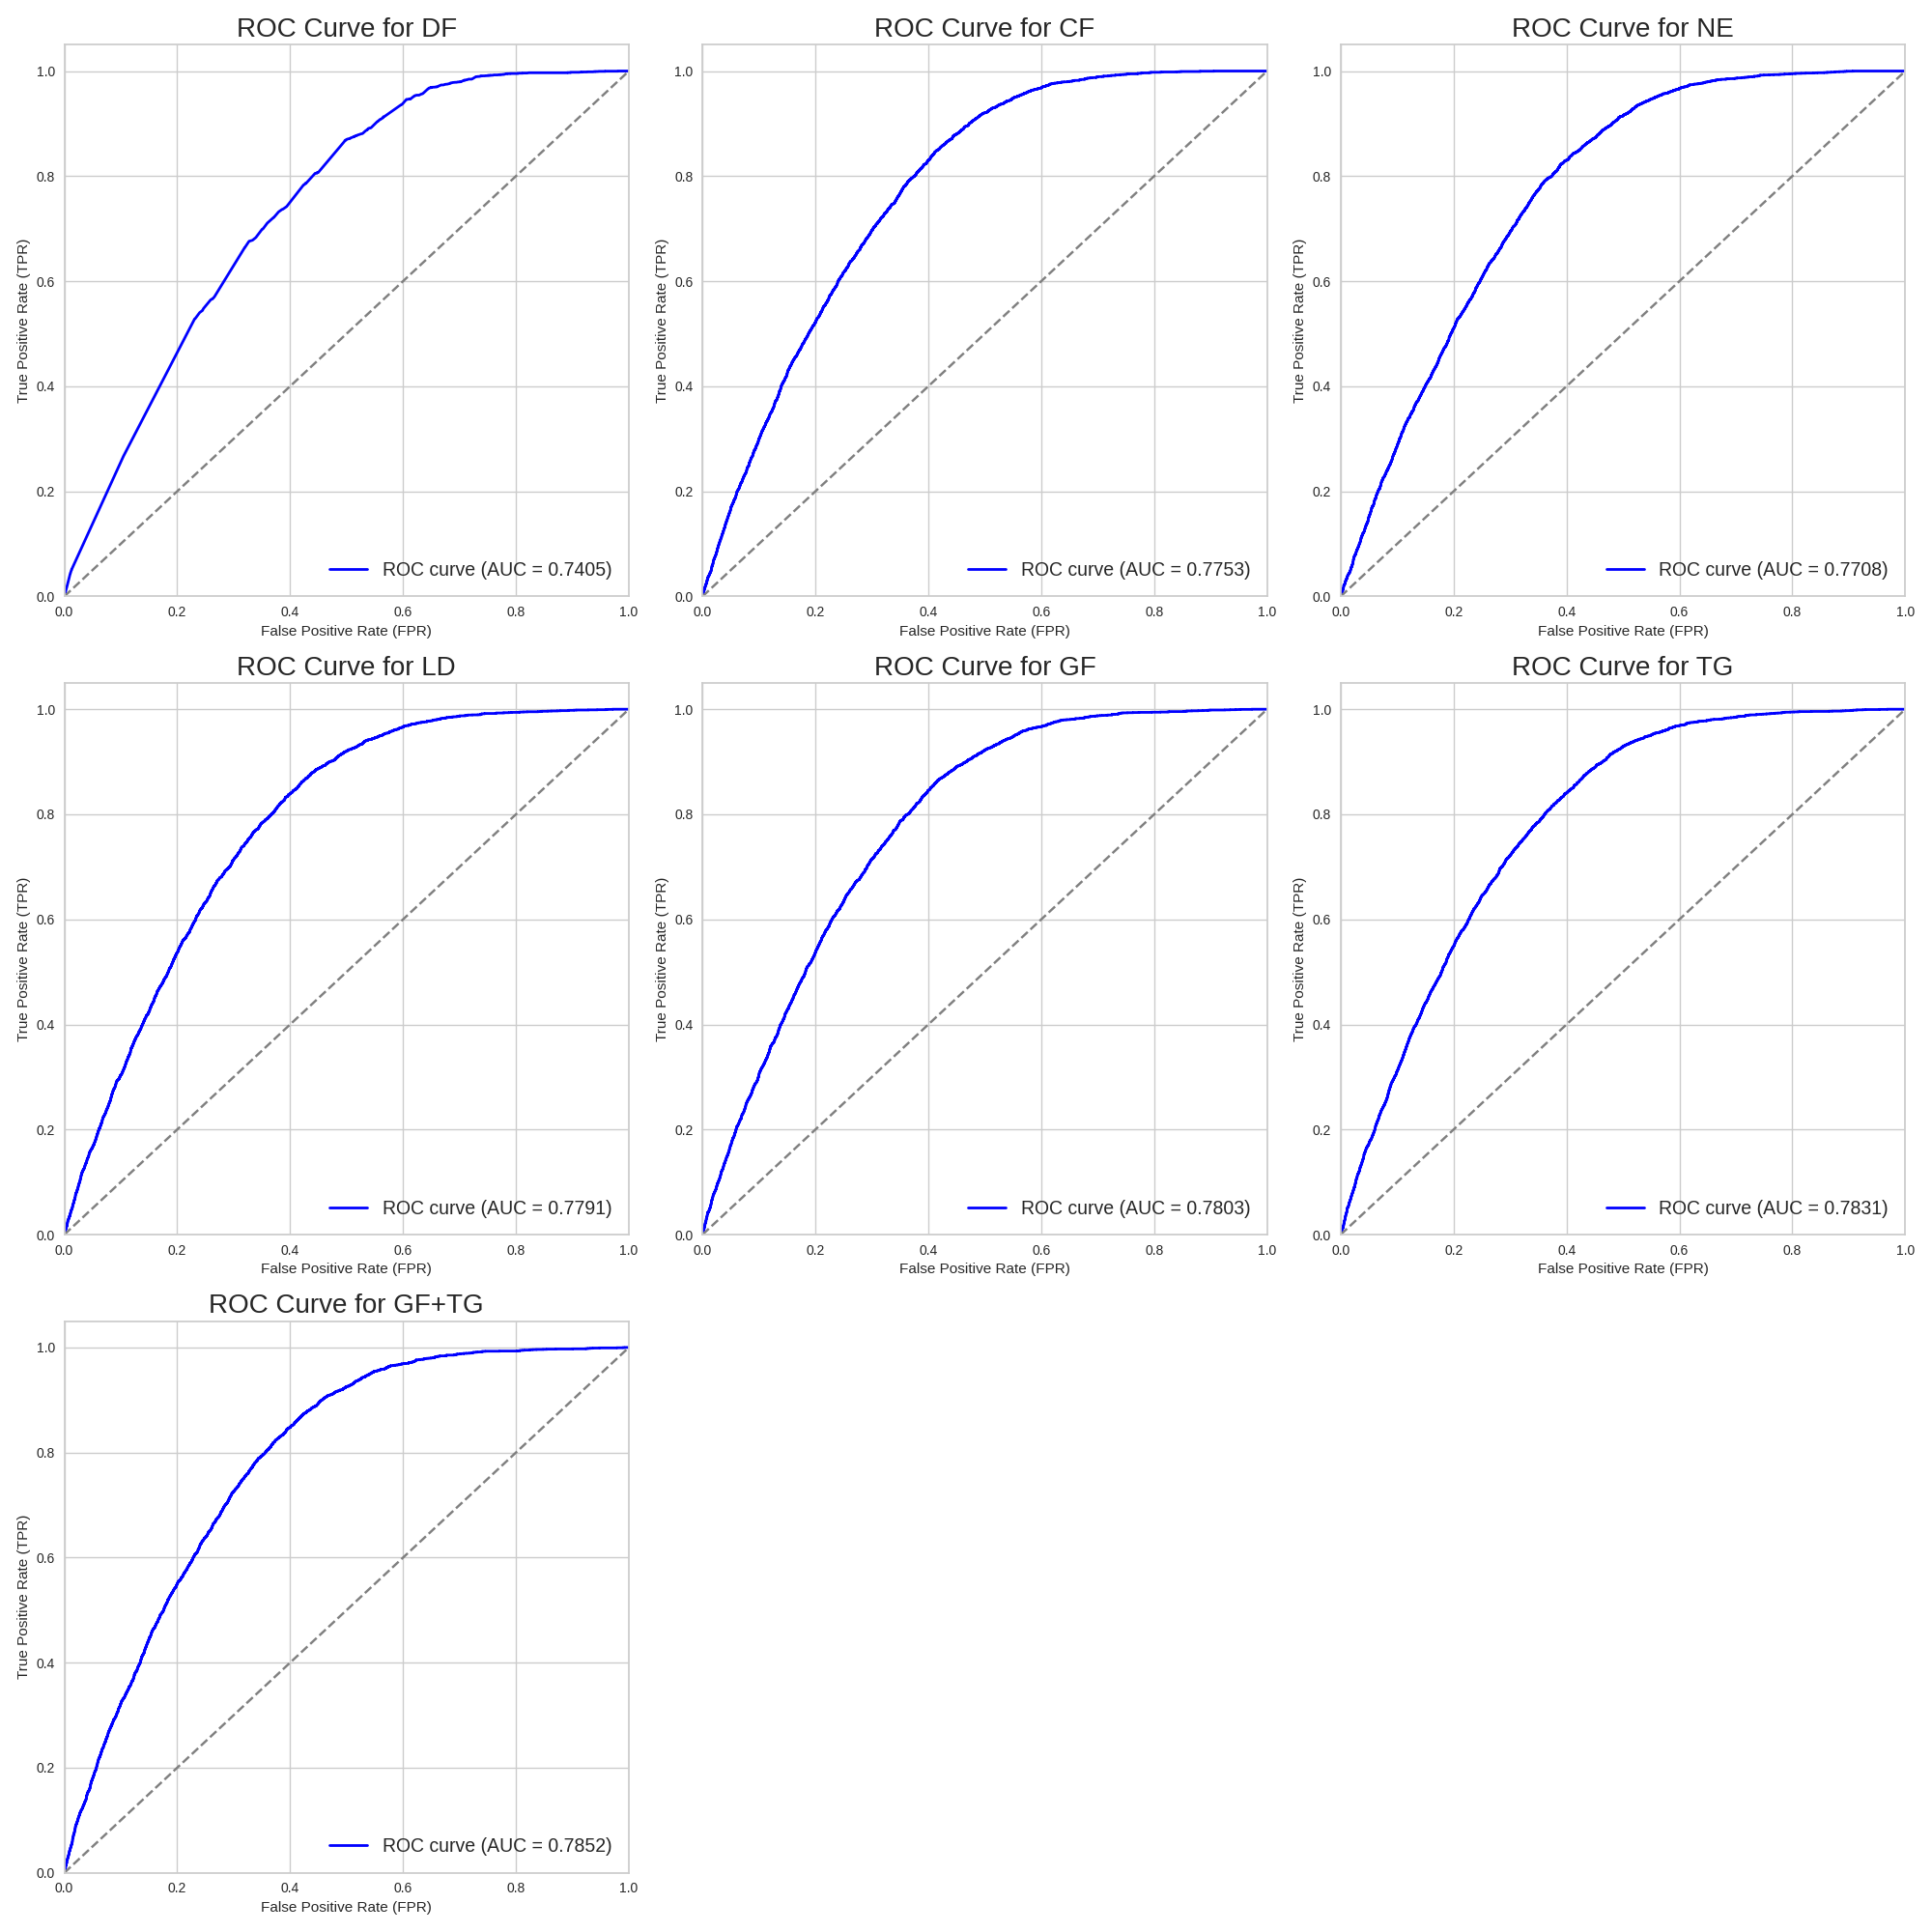
\includegraphics[scale=0.25]{./non-crime-no-timeseries-fig/roc_auc.png}
  \caption{ROC曲線}
  \label{fig:non-crime-no-timeseries-roc}
\end{figure}
%------------------------------------------
% table
%------------------------------------------
各モデルの予測精度を精度指標を基に比較した結果を表\ref{tb:non-crime-no-timeseries-index}にまとめる.
最も的中率が高いモデルはDFであるが,これは偽陽性を評価できていないのでPAIとAUCに注目する.
PAIについて注目すると,DFとCFの比較から特徴量を連続化すると大きな改善が確認できた.
また,距離特徴量を変換するNE,LD,GFではCFによる連続化と同等の改善がみられ,
GF+TGが最もPAIが高くなった.
AUCについて注目すると,DFと比較すると全てのモデルで同等の改善がみられ,
PAIと同様にGF+TGが最も高くなった.

また,DFとGF+TGのAUC値の有意差を評価するためにDeLong検定\citep{DeLong}を実施した結果,
p<0.001となり,両者のAUCに統計的に有意な差があることが確認できた.

\begin{table}[htbp]
  \centering
  \caption{各モデル間の精度比較}
  \begin{tabular}{l|r||r|r|r|r|r|r}
  \hline

モデル & DF & CF & NE & LD & GF & TG & GF+TG \\  \hline\hline
的中率 & \bf{50.2} & 30.7 & 30.3 & 34.4 & 34.1 & 38.1 & 36.9 \\ 
PAI & 1.93 & 2.35 & 2.28 & 2.36 & 2.36 & 2.40 & \bf{2.41} \\ 
AUC & 0.74 & 0.78 & 0.77 & 0.78 & 0.78 & 0.78 & \bf{0.79} \\ \hline


  \end{tabular}
  \label{tb:non-crime-no-timeseries-index}
\end{table}

\FloatBarrier